%% ~~~~~~~~~~~~~~~~~~~~~~~~~~~~~~~~~~~~~~~~~~~~~~~~~~~~~~~~~~~~~~~~~~ %%
%% ROV and AI synopsis + future steps document ~~~~~~~~~~~~~~~~~~~~~~ %%
%% Seattle Aquarium -- Benthic Resilience Project ~~~~~~~~~~~~~~~~~~~ %%
%% 1 Jan 2022 -- zhr ~~~~~~~~~~~~~~~~~~~~~~~~~~~~~~~~~~~~~~~~~~~~~~~~ %%
%% ~~~~~~~~~~~~~~~~~~~~~~~~~~~~~~~~~~~~~~~~~~~~~~~~~~~~~~~~~~~~~~~~~~ %%





%% preamble: load packages / document settings ~~~~~~~~~~~~~~~~~~~~~~ %%
\documentclass[11pt]{article}
\usepackage[dvipsnames]{xcolor}
\usepackage[position=top]{subcaption}
\captionsetup[subfigure]{skip=0pt}
\usepackage{float}
\floatstyle{plaintop}
\restylefloat{table}
\usepackage{graphicx}
\graphicspath{{./figs/}}
\usepackage[export]{adjustbox}
\usepackage{caption}
\usepackage{subcaption}
\usepackage{wrapfig}
\usepackage{setspace} 
\usepackage{ragged2e}
\usepackage[margin=1in]{geometry}
\usepackage[hypertexnames=false]{hyperref}
\hypersetup{urlbordercolor=blue}
\hypersetup{linktocpage=true}
%% END preamble ~~~~~~~~~~~~~~~~~~~~~~~~~~~~~~~~~~~~~~~~~~~~~~~~~~~~~ %%





%% custom commands ~~~~~~~~~~~~~~~~~~~~~~~~~~~~~~~~~~~~~~~~~~~~~~~~~~ %%
\newcommand{\w}{.33\textwidth} % set figure width 
\newcommand{\h}{.27\textwidth} % set figure height
\newcommand{\ww}{.5\textwidth} % set 2nd figure width
\newcommand{\hh}{.31\textwidth} % set 2nd figure height  
\newcommand{\pt}{\vspace{-.5em}} % reduce vertical spacing 
%% END custom commands ~~~~~~~~~~~~~~~~~~~~~~~~~~~~~~~~~~~~~~~~~~~~~~ %%





%% title page and title information ~~~~~~~~~~~~~~~~~~~~~~~~~~~~~~~~~ %%
\title{
Remotely Operated Vehicle (ROV) and Artificial Intelligence (AI) test 
results, current status, and future action items
}
\author{
Zachary Randell, Research Scientist
\\
Alex Tanz, Marine Science Interpreter \& Diver 
\\
Shawn Larson, Curator of Conservation Research
\\
\vspace{5pt}
\textit{\textbf{Conservation Programs \& Partnerships, Seattle 
Aquarium}}
}
\begin{document}
\begin{titlepage}
\maketitle
\tableofcontents
\vfill
\centering

\includegraphics[width=3cm]{logo.jpg}
\\
\textit{\textbf{
Climate Resilience $\vert$ 
Sustainable Seas $\vert$ 
Clean Waters
}} 
\vfill
\justifying
\noindent\textit{Note to the reader}: this pdf is from a LaTeX 
document that contains embedded links, both 
within (red border, e.g., Fig.~\ref{fig:ROVdev}, for figures and 
sections) and 
external (blue border, e.g.,  
\href{https://www.latex-project.org/about/}{url}, 
for relevant websites and videos in Google Drive). 
When viewing this document offline (e.g., in an adobe reader after 
downloading the file), if you click on a red box to jump to a figure or 
section, click and hold \textit{Alt} then \textit{left-arrow} (on PC) 
or \textit{Command} then \textit{left-arrow} (on Mac) to return to your 
previous page in the document.
\end{titlepage}
%% END title page~~~~~~~~~~~~~~~~~~~~~~~~~~~~~~~~~~~~~~~~~~~~~~~~~~~~ %%





%% begin document ~~~~~~~~~~~~~~~~~~~~~~~~~~~~~~~~~~~~~~~~~~~~~~~~~~~ %%
\section{Abstract}
\label{Abstract}
Our objective is to use the emerging accessibility of Remotely Operated 
Vehicle (ROV) technology and Artificial Intelligence (AI) software to 
expand the spatial extent across which we can make inferences about 
patterns of benthic community structure. 
When nested within a long-term subtidal monitoring program, we envision 
such advancements in survey and processing methodology will enhance our 
ability to identify the processes and factors affecting ecological 
resilience and kelp-forest persistence through time.
In order to provide scientific SCUBA divers an additional benthic 
survey tool, we are testing and developing ROV methods to survey 
relatively shallow (5-40m) locations characterized by urchin barrens, 
and turf, understory, and canopy forming macroalgae. 
Given the large amount of imagery envisioned, we are training 
AI algorithms to generate estimates of percent-cover and object 
(species) abundances at scale.
  
Regarding current status, we have tested the Seattle Aquarium's 
\href{https://bluerobotics.com/wp-content/uploads/2020/02/br_bluerov2_datasheet_rev6.pdf}{Blue
 ROV2} on four separate occasions.
These tests have largely centered around iterating camera and light 
placement, and we have developed a custom framework upon which to mount 
the ROV's lights. 
On the AI side, we have established pipelines using 
\href{https://coralnet.ucsd.edu/blog/a-new-deep-learning-engine-for-coralnet/}{CoralNet}
 to analyze percent-cover from photos, and 
\href{https://www.viametoolkit.org/}{VIAME} to detect objects 
(individuals of conspicuous species) from photos/video. 
%Having secured preliminary funding from the Sea Otter Foundation and 
%Trust \href{https://seaotterfoundationtrust.org/}{(SOFT)} and the 
%North 
%Pacific Coast Marine Resources Committee 
%\href{https://www.jeffersoncountypublichealth.org/1523/North-Pacific-Coast-Marine-Resources-Com}{(NPC
% MRC)}, the Seattle Aquarium will launch this project 1st quarter 
%2022. 
Our immediate next steps involve developing standardized ROV survey 
protocols and full-scale establishment/testing of AI pipelines. 
We envision a highly collaborative project, thus this document is 
intended to set the stage for transparent and reproducible research;
open dialogue---your thoughts, feedback, and criticisms---are most 
welcome.  
%% END abstract ~~~~~~~~~~~~~~~~~~~~~~~~~~~~~~~~~~~~~~~~~~~~~~~~~~~~~ %%





%% Begin ROV tests ~~~~~~~~~~~~~~~~~~~~~~~~~~~~~~~~~~~~~~~~~~~~~~~~~~ %%
\section{ROV testing}
We have tested the ROV on four occasions, with a single $1hr$ dive each 
of the four days. 
Major points from each of the four days are noted below, and this 
section closes with an itemized breakdown of future ROV tasks. 
Finally, big shoutout to Alex Tanz at the Seattle Aquarium for leading 
the assembly and initial wiring of the ROV, as well as for assisting in 
all ROV tests that took place at the Seattle Aquarium. 

\subsection{\textit{September 1st}}
We calibrated ROV controls in a holding tank prior to our first flight 
off the side of the Seattle Aquarium down to 70$'$ 
(Fig~\ref{fig:ROVdev}\textit{a}). 
Controlling the ROV via a Xbox game controller was intuitive and the 
ROV was very responsive, particularly when ``feathering" the controls, 
i.e., the ROV was responsive to varying strengths of thruster 
(joystick) input. 
The 
\href{https://bluerobotics.com/learn/bluerov2-software-setup/}{QGroundControl}
 software (QGC) that communicates with the ROV was easy to install and 
 can be readily accessed to download logs of ROV activity.
No GoPros were used during this first flight.
	
\subsection{\textit{November 10th}}
In a first test of the ``benthic camera array," two GoPro HERO 10 
cameras were mounted on the 
\href{https://www.bluerobotics.com/store/rov/bluerov2-accessories/brov-payload-skid/}{payload
 skid} underneath the ROV (Fig~\ref{fig:ROVdev}\textit{b}), and a third 
GoPro was staged behind the other two and faced forwards.
Of the two benthic-facing cameras, one recorded 4K 120FPS (frames per 
second) video, the other shot 23MP (megapixel) photos every 2 seconds.
We once more deployed the ROV off the side of the Seattle Aquarium. 
	
We anticipate sharing the live-feed of the ROV will be an invaluable 
tool for public outreach and education, particularly for 
classroom/field trip events with communities along the coast and in 
Puget Sound, and also as an additional tool to engage visitors at the 
Seattle Aquarium. 
In order to evaluate the ease of sharing the real-time ROV feed, Alex 
set up a TV, connected it to the ROV laptop, and streamed video from 
the forward-facing (built-in) camera used to steer the ROV. 
We also initiated a Zoom meeting from the dedicated ROV laptop, 
screen-shared, and had Seattle Aquarium personnel in another building 
open the meeting and view the live ROV video. 
We are now exploring how to directly connect the ROV video feed as a 
webcam, i.e., using the ROV camera's IP address. 
Additional software is required to make this happen, and doing so will 
provide higher quality video that avoids double-compression in QGC and 
Zoom. 
In essence, we want a separate video stream that bypasses QGC and 
goes straight to Zoom, or whatever other media outlet source is 
desired, e.g., a local TV. 
		
The benthic camera array worked well in terms of \textit{obtaining} 
video and time-lapse photos. 
However, as you can see in Fig~\ref{fig:images}\textit{a---c}, a shadow 
is prominent in the middle of the frame, and the left-third
of the frame is not well illuminated. 
These lighting effects were not a surprise given that the light 
configuration on Nov 10th was the ``default" configuration, which 
maximizes light illumination directly in front of (and not below) the 
ROV (Fig.~\ref{fig:ROVdev}\textit{b}).
Despite suboptimal lighting, the latest-generation GoPros 
demonstrated a high-degree of adaptability to light variability, and the
image-stabilization performed extremely well. 
You can see this in 
\href{https://drive.google.com/file/d/1RKhWZ2E1E4xGpWKGdaA42evfIxkJVx0c/view?usp=sharing}{Vid~1.},
 a short video from the benthic-facing camera. 
This is a 4K video, though your media player will downscale it, 
particularly when viewing the clip in Google Drive (though you can 
download the original 4K file). 
	
\subsection{\textit{November 12th}}
Following November 10th's test and the presence of shadows/suboptimal 
illumination, I changed light placement such that the lower of the two 
lights were attached to the payload skid (a relatively small 
adjustment). 
I traveled to Whidbey Island where Ken Collins was kind enough to host 
and take me and the ROV out on his vessel. 
We launched out of Freeland County Park, anchored at the northeast 
corner of Holmes Harbor 
(\href{https://www.whatsmygps.com/?lat=48.085055555555556\&lng=-122.52177777777777}
{$48^\circ$ $5'$ $6.2016''$ N, $122^\circ$ $31'$ $18.4002''$ W}),
 and flew the ROV above an eelgrass bed, and along soft sediment down 
 to 85$'$ (Fig.~\ref{fig:images}\textit{d---f}, 
\href{https://drive.google.com/file/d/1Ure4E4GWHOEm1omK0y09ecN_KXguUfjQ/view?usp=sharing}{Vid.~2}).

Regarding lighting, while I succeeded at providing more uniform 
lighting across the camera's field of view, I inadvertently also 
succeeded at creating a large amount of backscatter by illuminating the 
water column underneath the cameras. 
For example, note how the image with eelgrass appears out of focus 
(Fig.~\ref{fig:images}\textit{f}) relative to photos from Nov 10th 
(Fig.~\ref{fig:images}\textit{a---c}).
Furthermore, in 
\href{https://drive.google.com/file/d/1Ure4E4GWHOEm1omK0y09ecN_KXguUfjQ/view?usp=sharing}{Vid.~2})
note the faint, approximately biradial shadow present  
(most visible in the short clips along soft sediment); 
this stemmed from the light's beam hitting the frame upon which the 
lights were mounted.

Others lessons from Nov 12th: the ROV performed well in a moderate 
current. 
In particular, the software governing ROV movement compensates 
incredibly well for the varying forces acting upon ROV position at any 
one point in time. 
BUT, despite being able to point the ROV towards a heading 
(via the compass on our laptop display), current still had a 
significant effect upon realized ROV position, e.g., flying the ROV 
north with a current running west does not put the ROV where one 
expects it to be.
This first field deployment away from the relative shelter of the 
Seattle Aquarium illustrated the importance of incorporating an 
acoustic GPS 
tracking system into our ROV operations. 
Such a tracking system will provide explicit knowledge of---and control 
over---ROV position, crucial for basic operations and the execution of 
repeatable (i.e., consistent survey location) and standardized 
(consistent area covered) benthic surveys. 

\begin{figure}[h!]
\centering
\subfloat[]{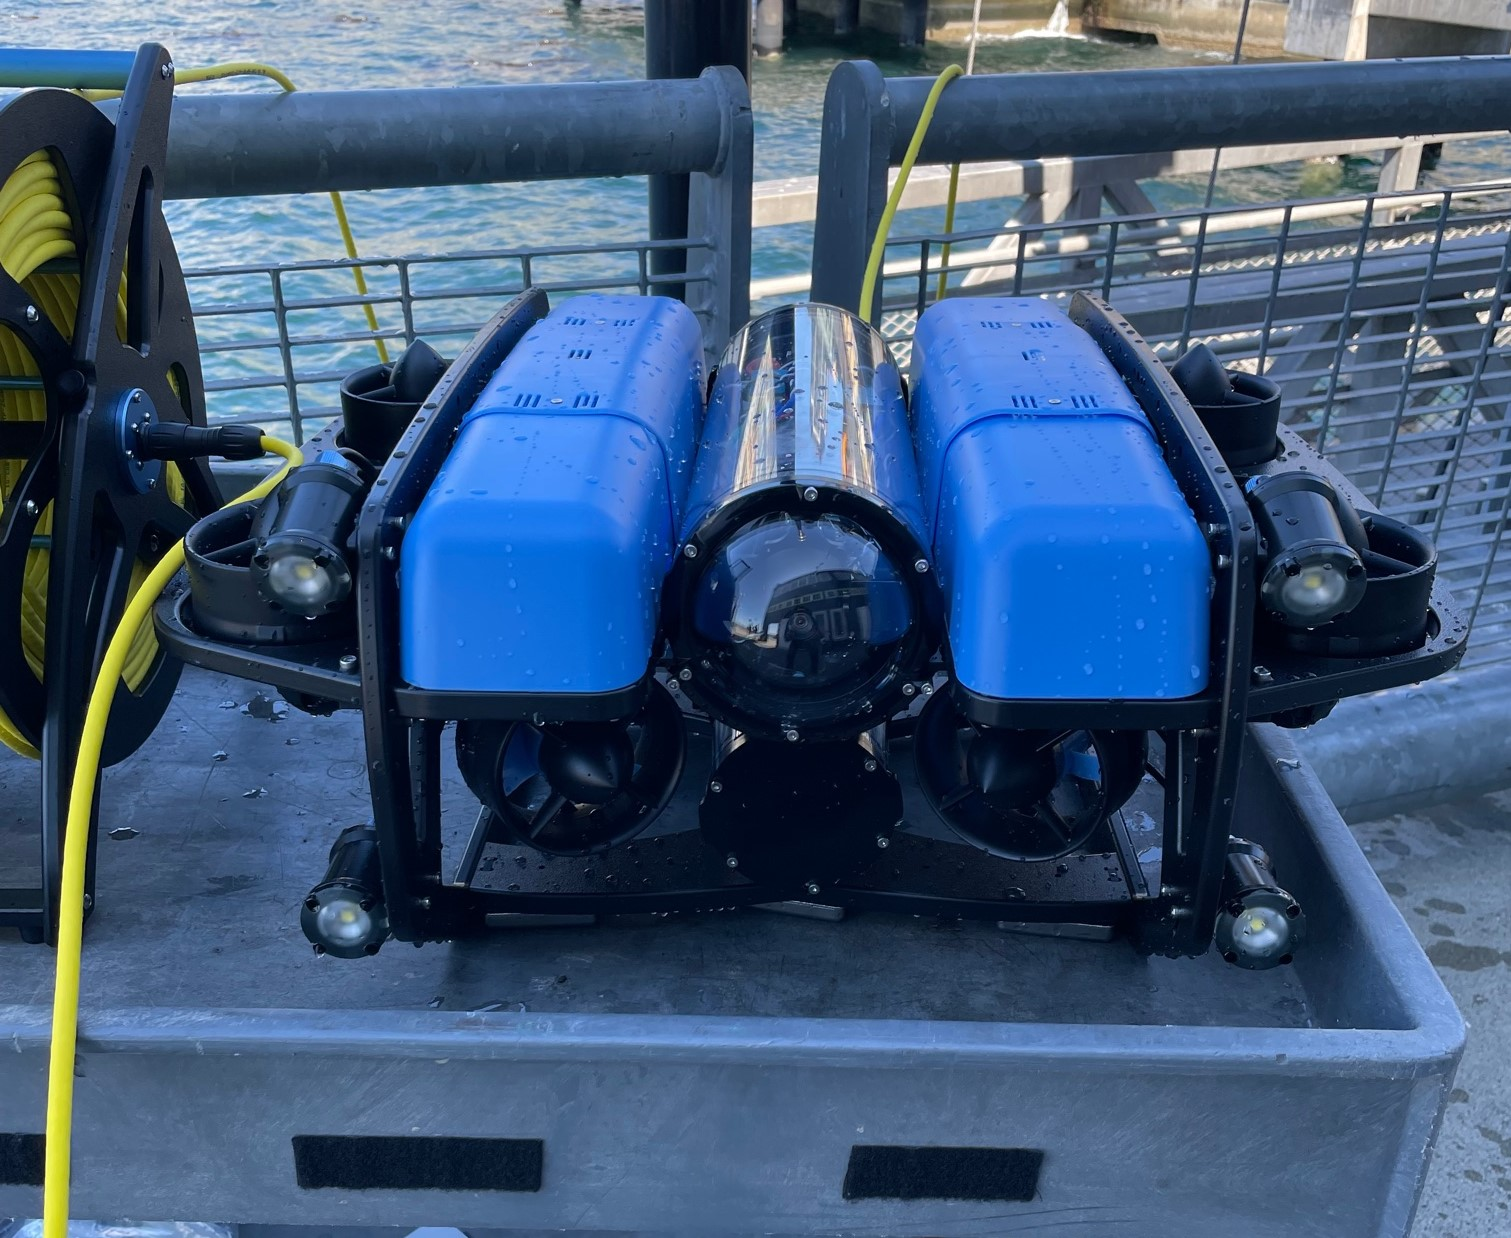
\includegraphics[
width=\w, height=\h, valign=t]{ROV1.jpg}}
\subfloat[]{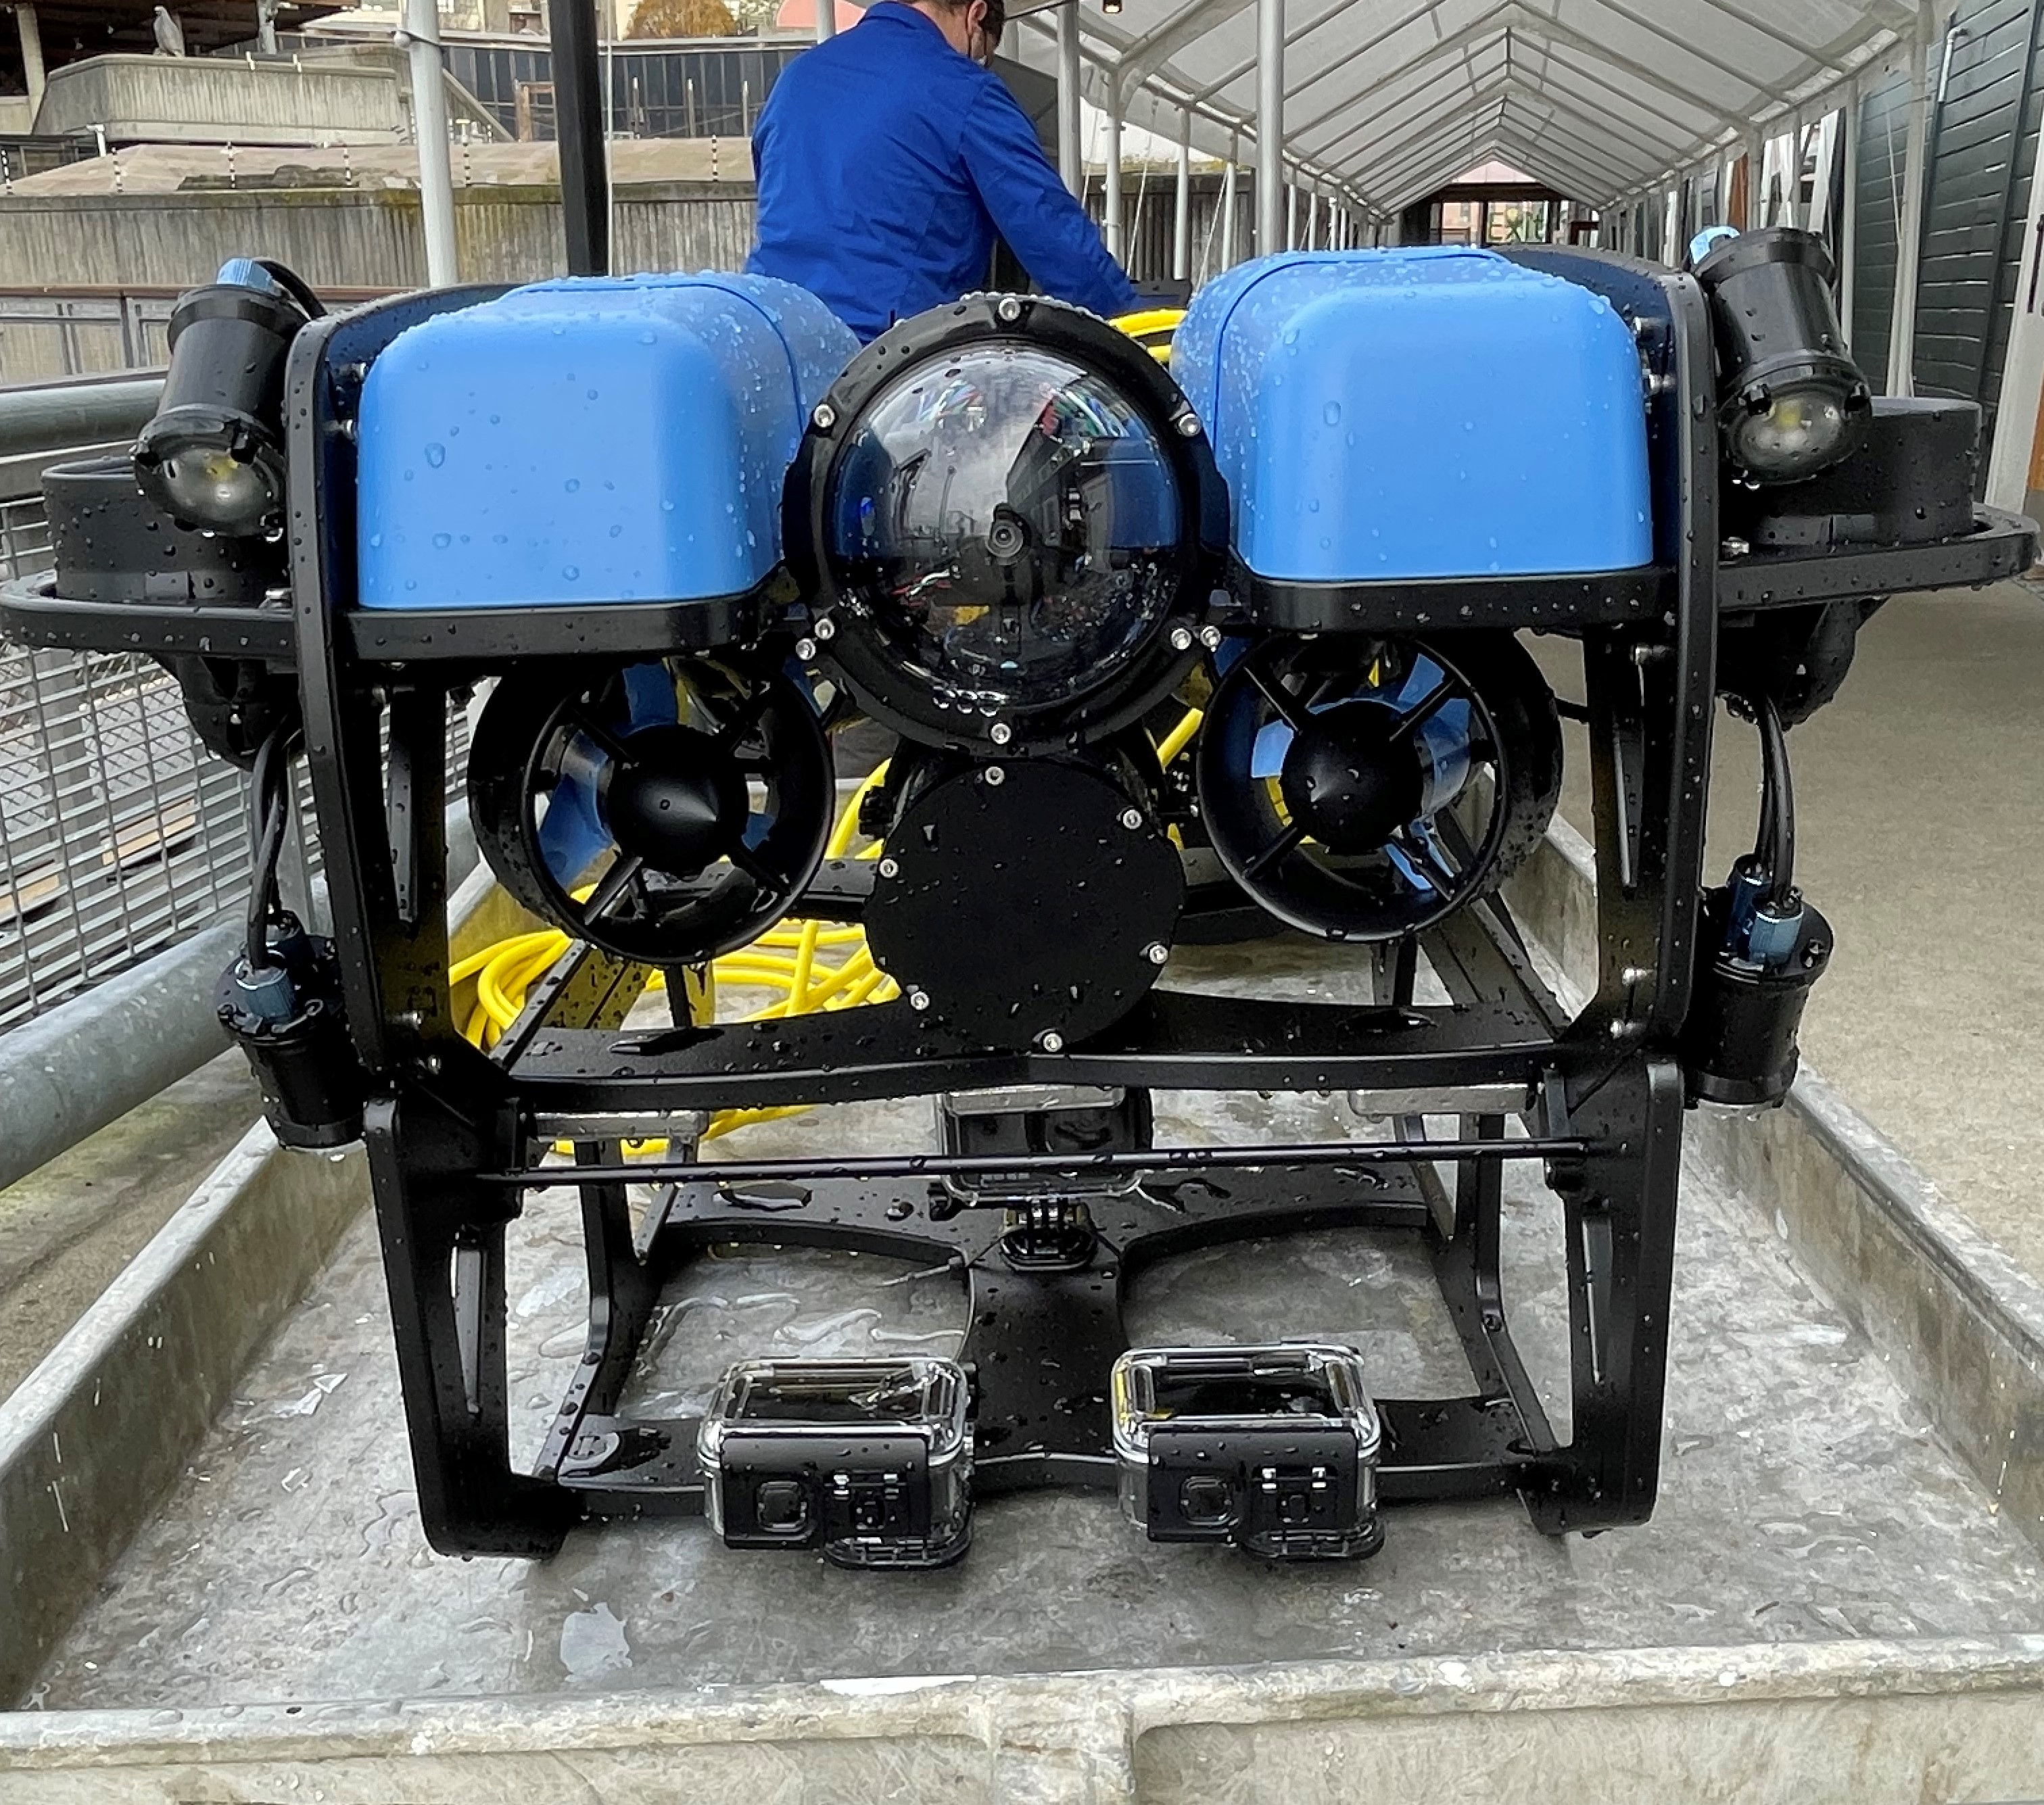
\includegraphics[
width=\w, height=\h, valign=t]{ROV2.jpg}}
\subfloat[]{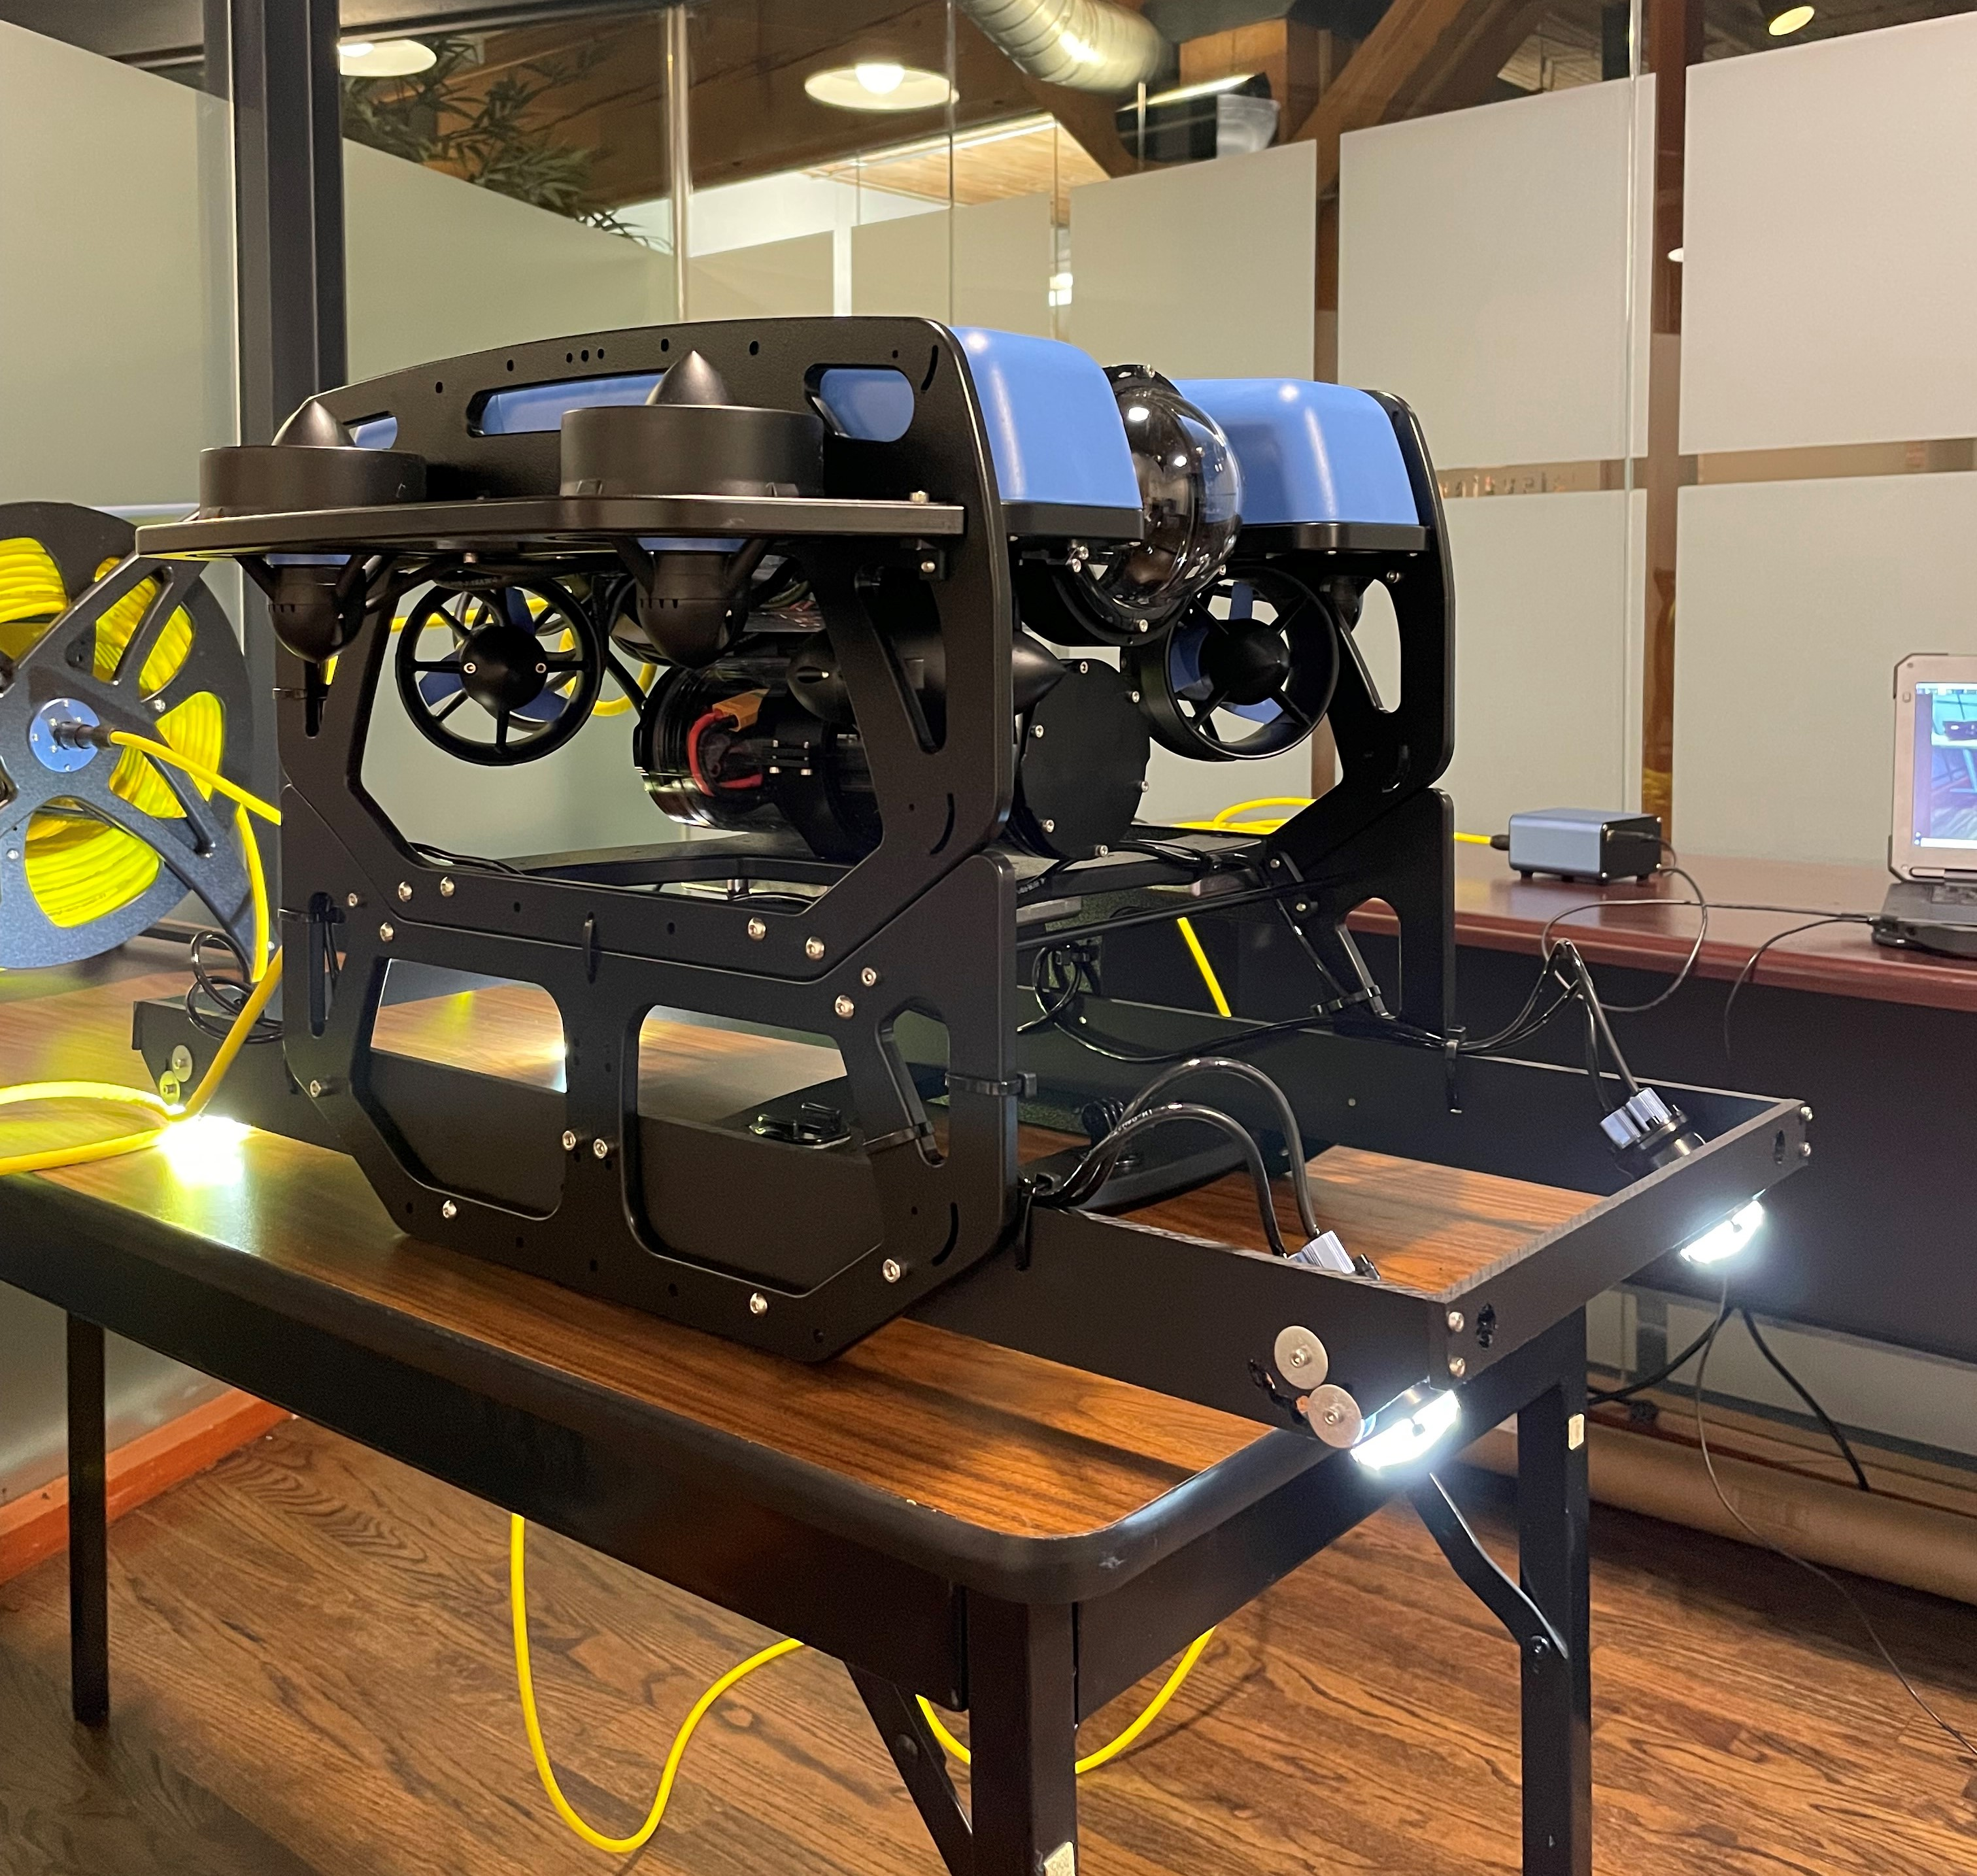
\includegraphics[
width=\w, height=\h, valign=t]{ROV3.jpg}}
\\
\subfloat[]{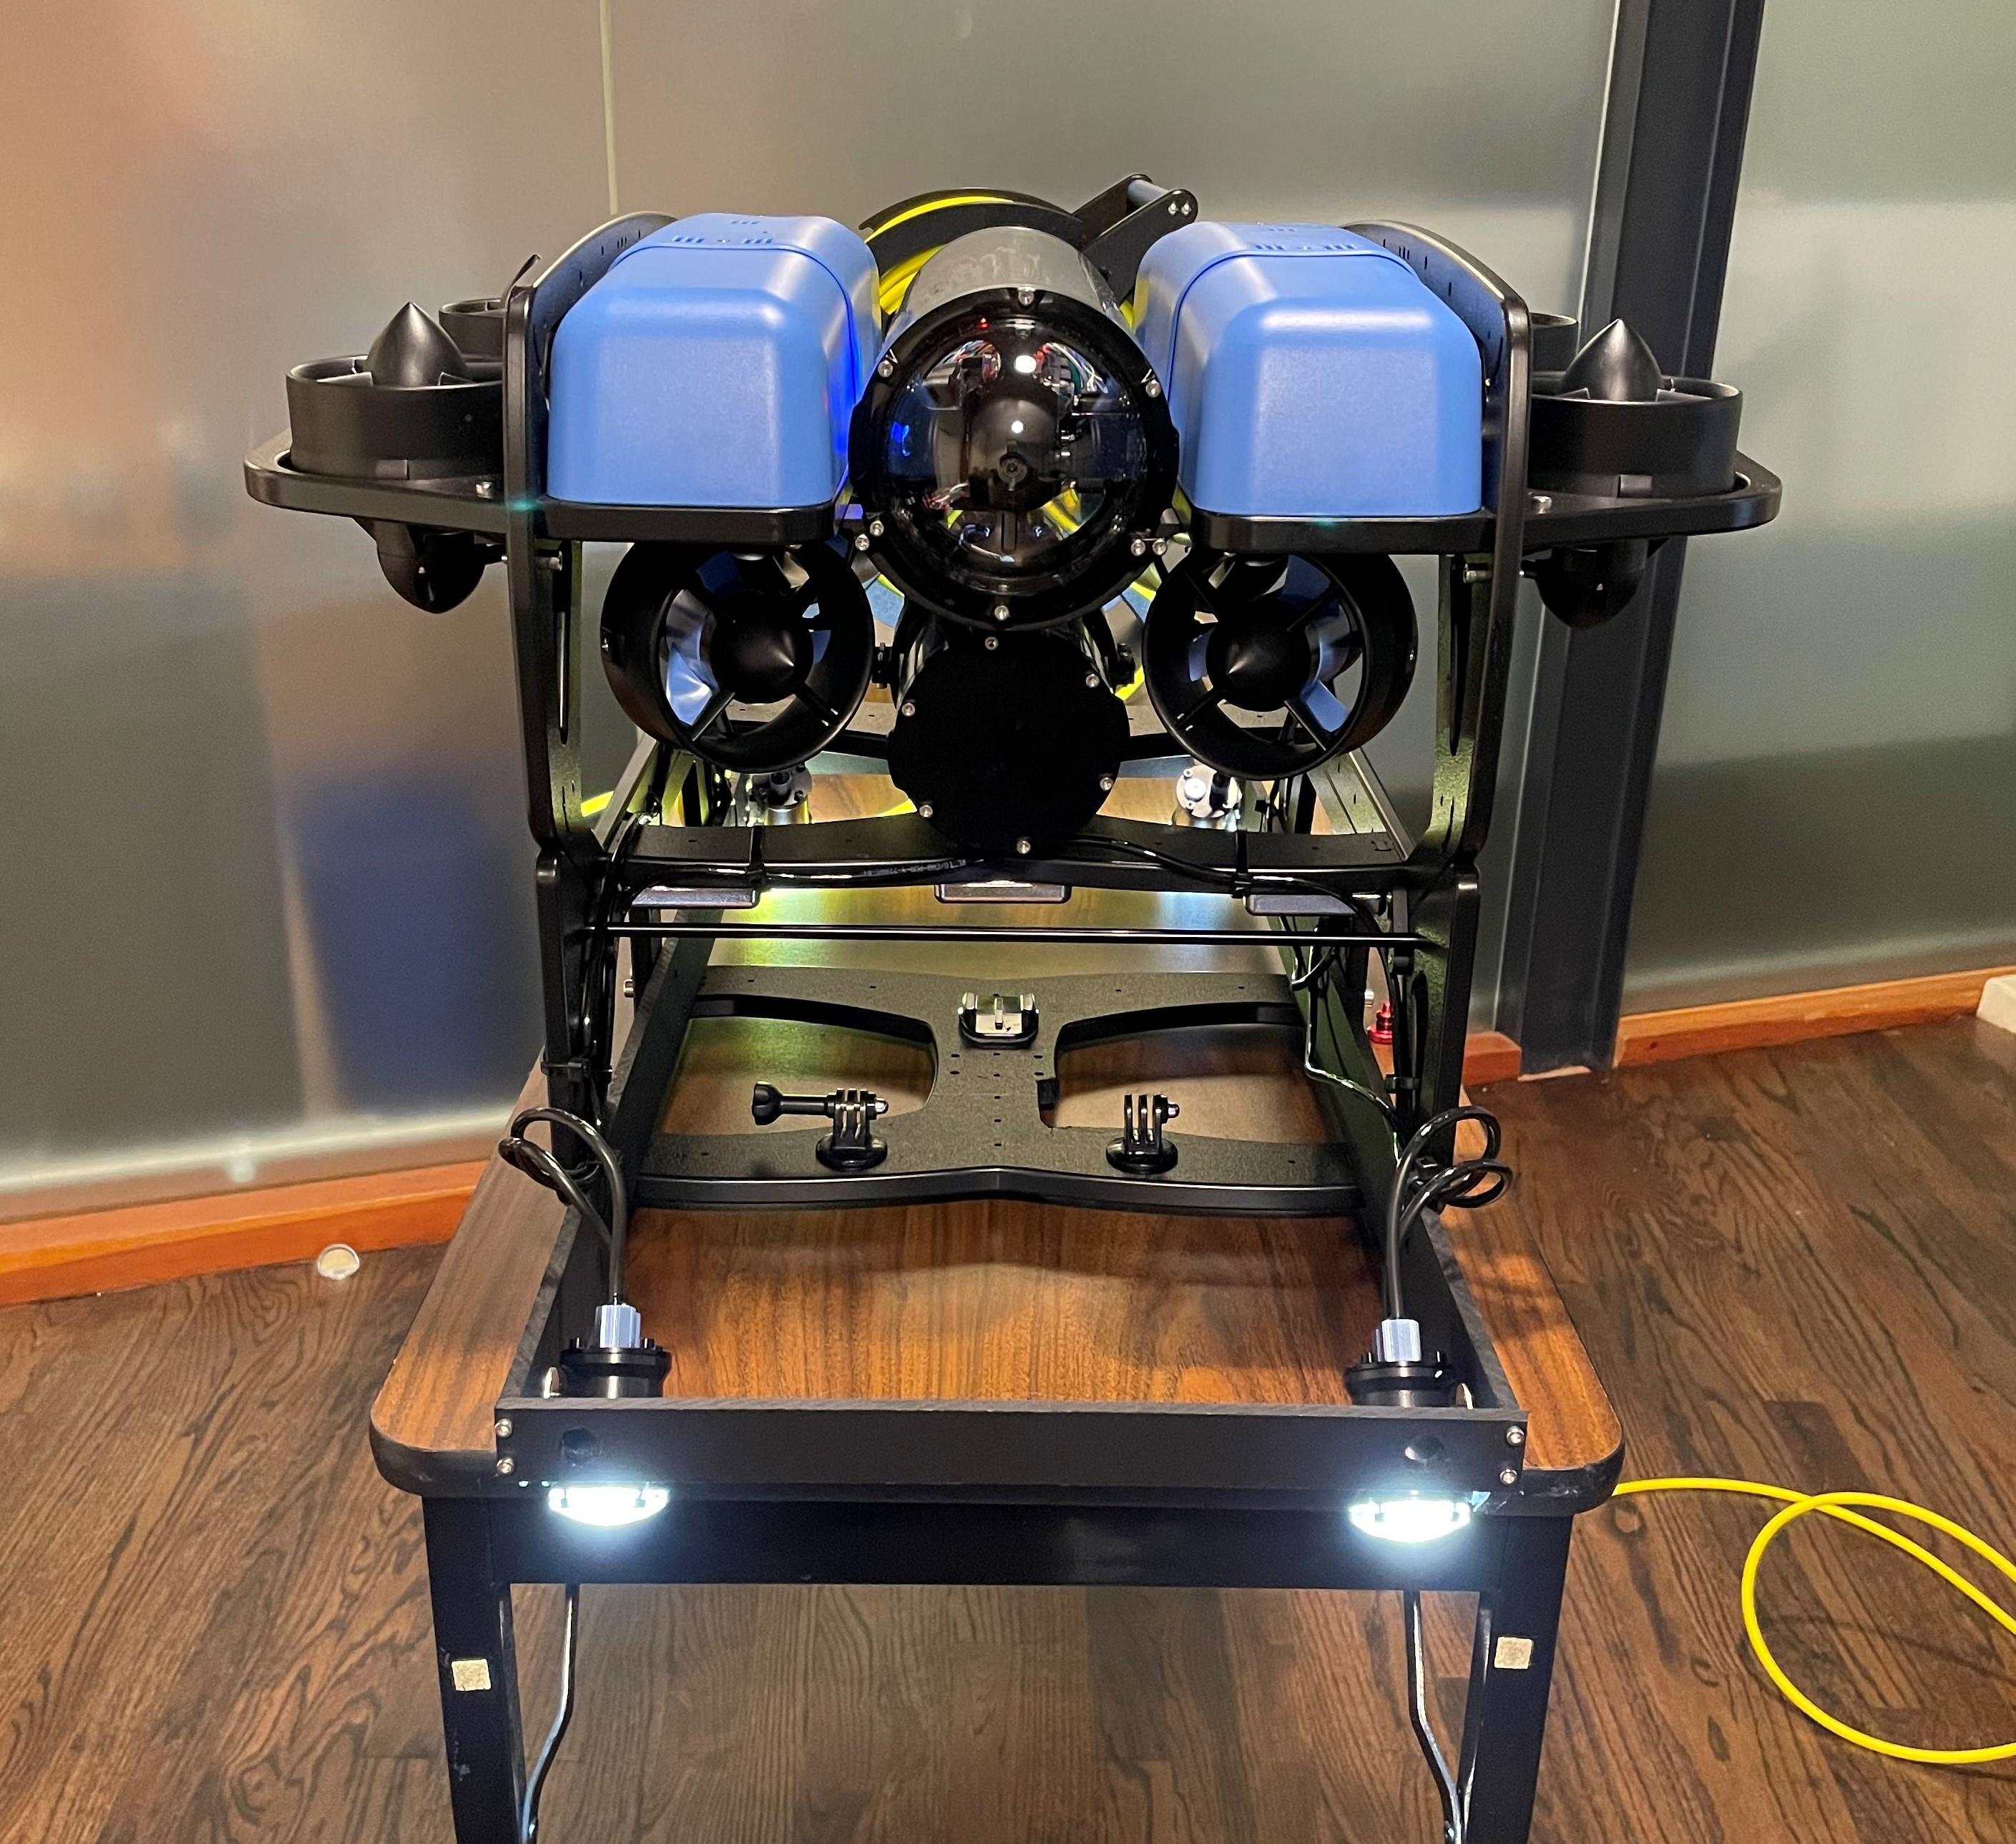
\includegraphics[
width=\w, height=\h, valign=t]{ROV6.jpg}}
\subfloat[]{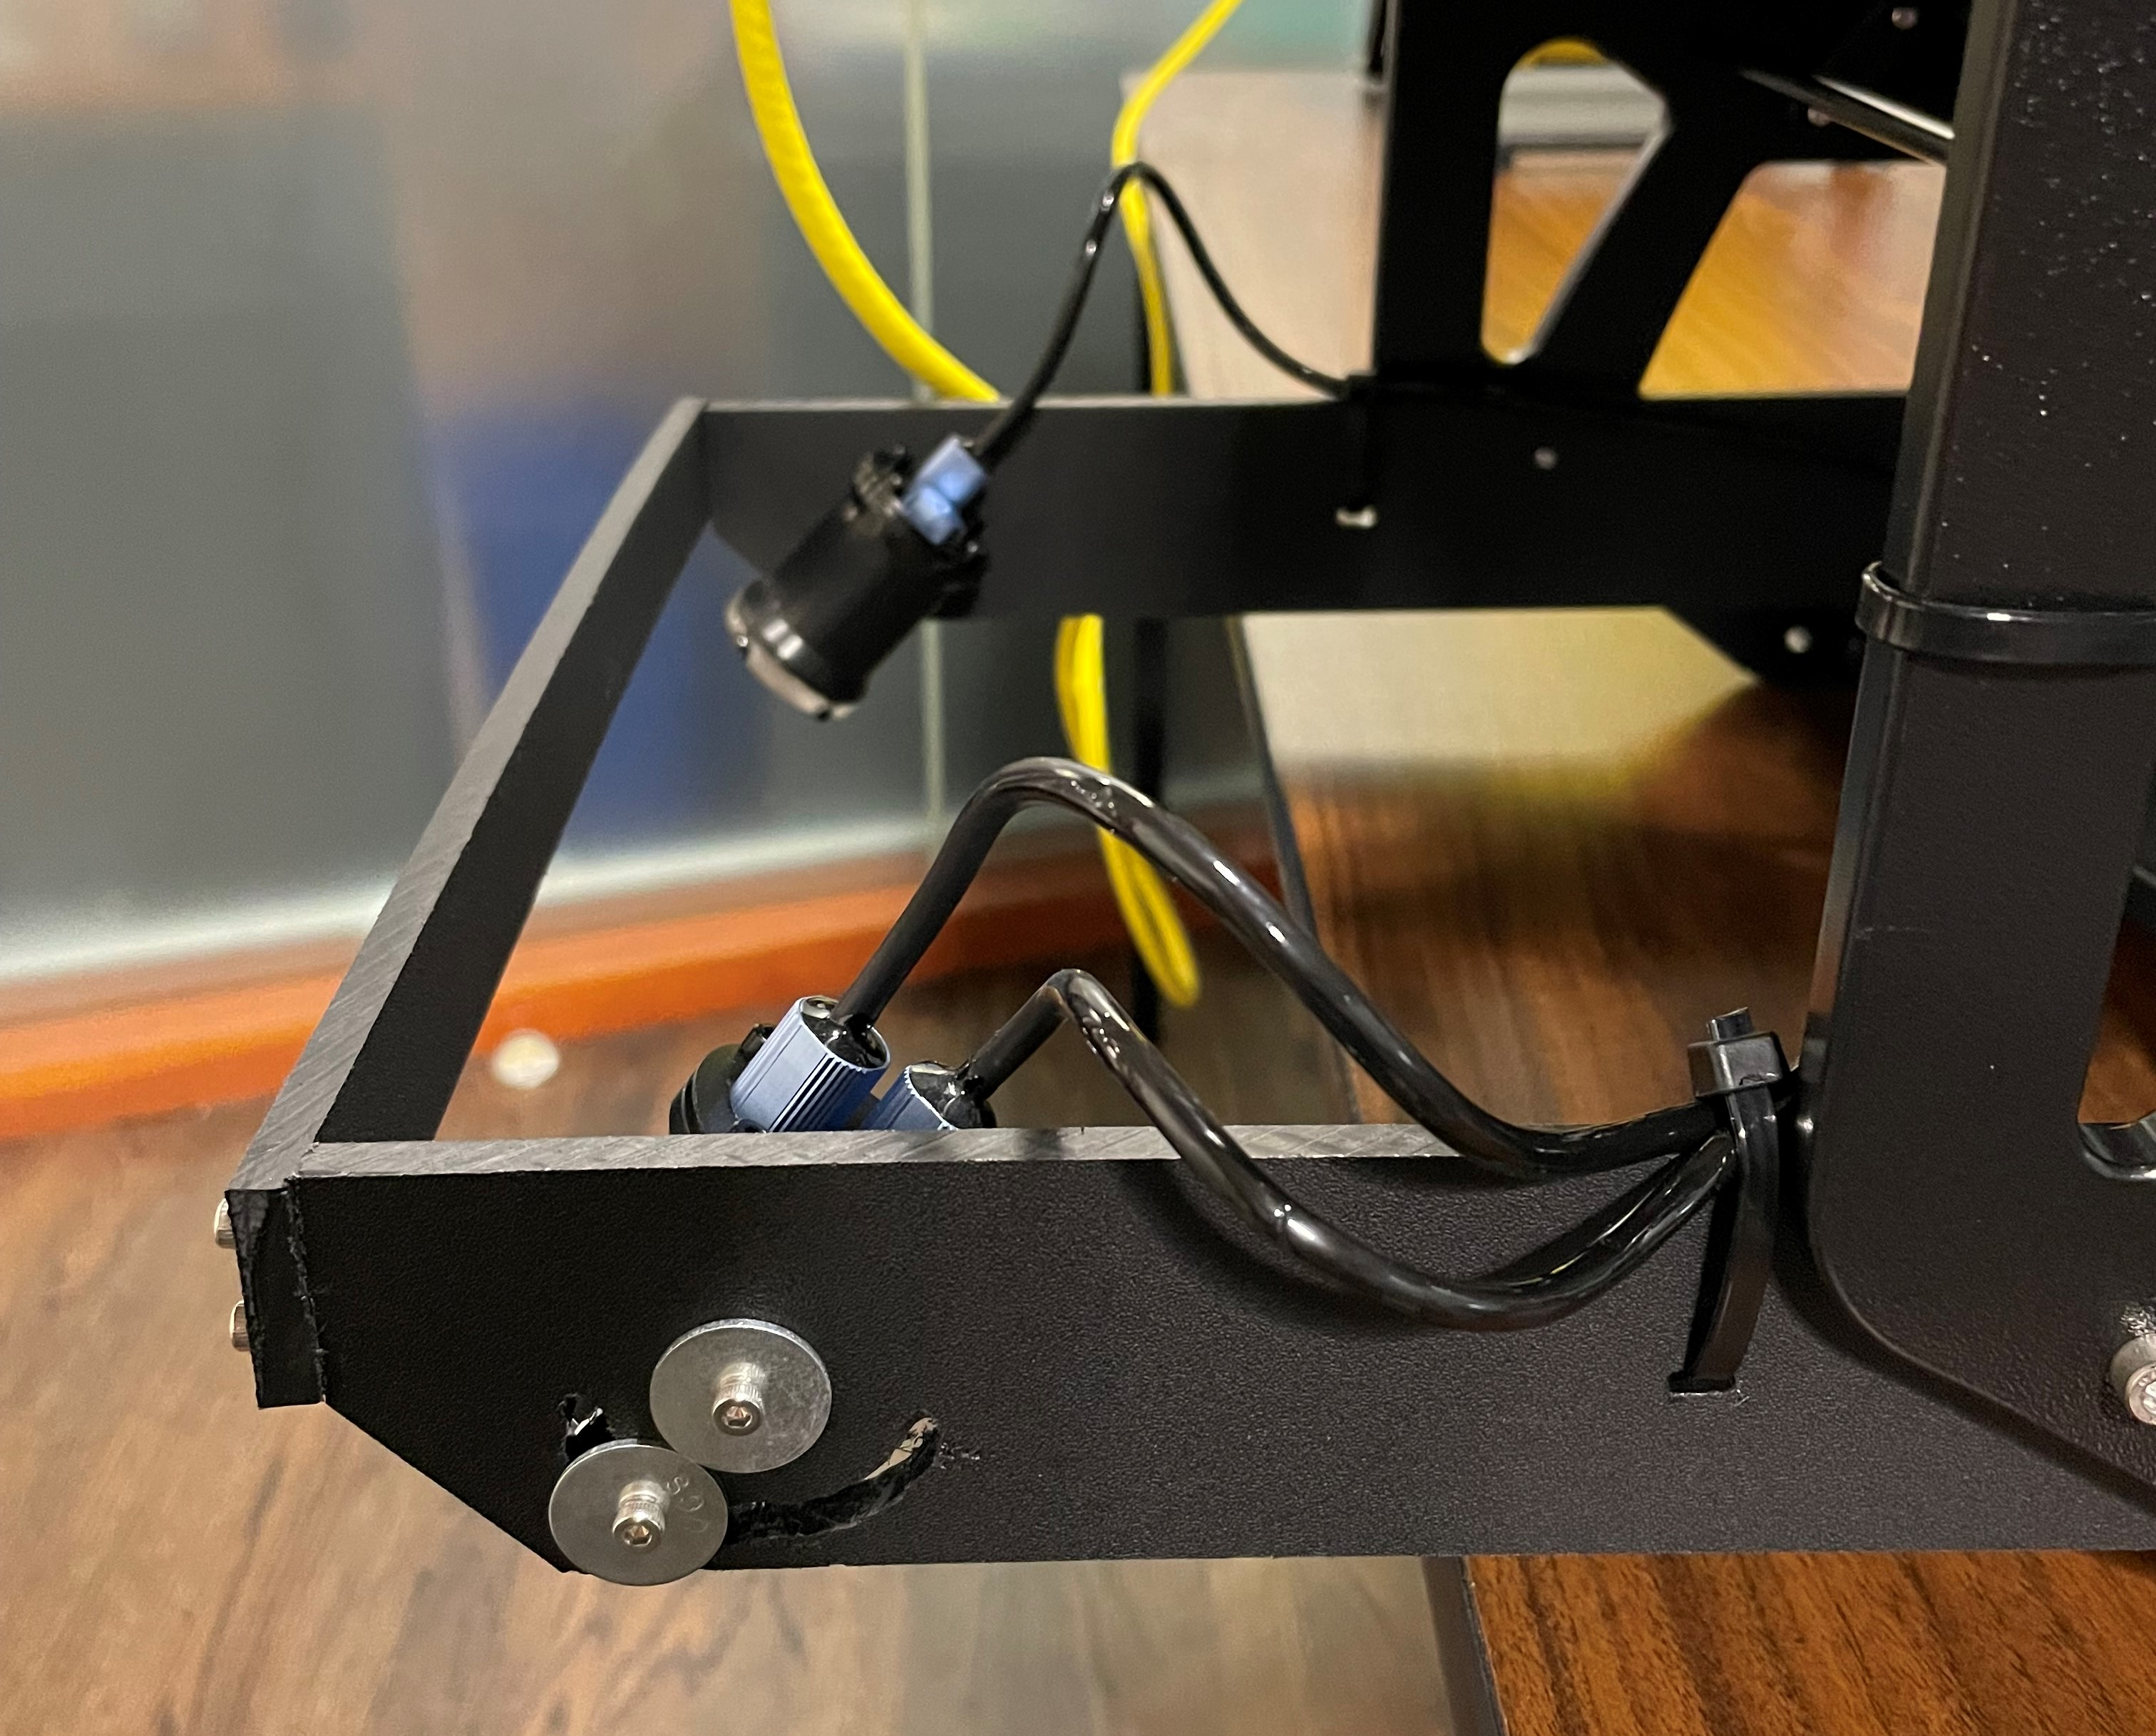
\includegraphics[
width=\w, height=\h, valign=t]{angle.jpg}}
\subfloat[]{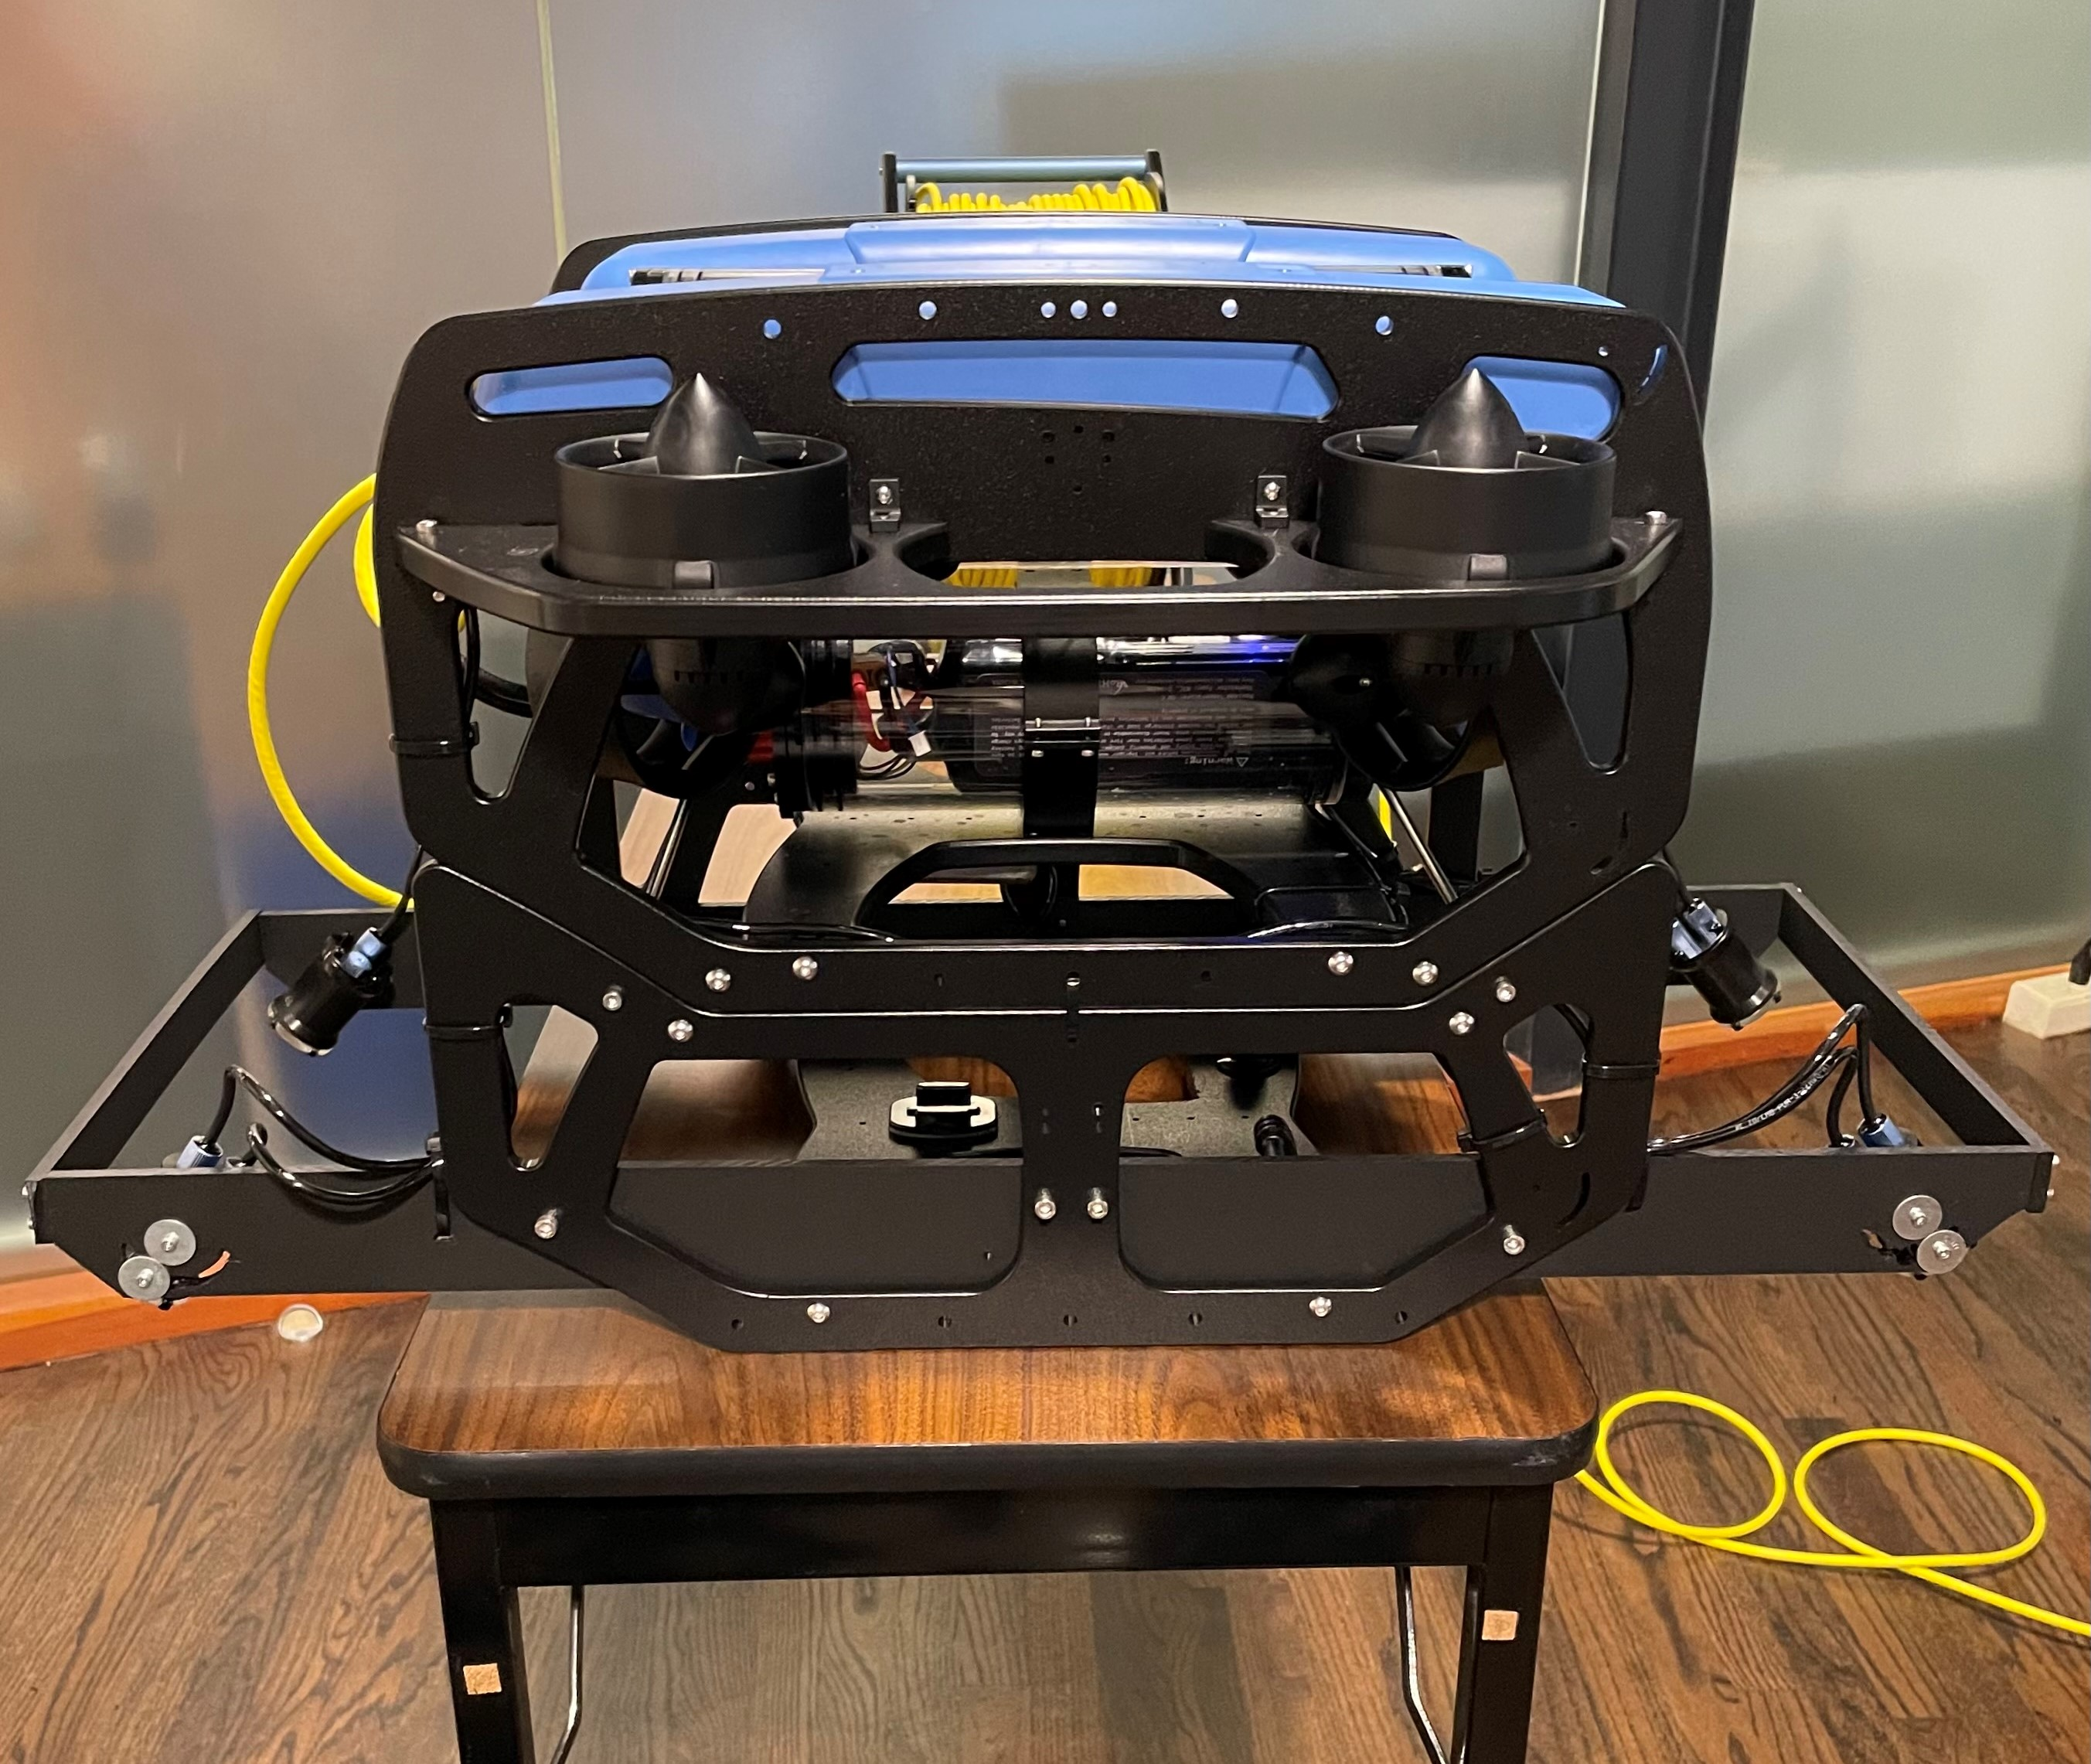
\includegraphics[
width=\w, height=\h, valign=t]{side.jpg}}
\caption{
(\textit{a}) The ROV as it was flown Sep 1st following assembly. 
(\textit{b}) Nov 10th we added the payload skid underneath the ROV, 
along with two GoPro HERO 10 cameras facing downwards. 
(\textit{c}) The current version of the ROV includes HDPE panels 
constructed to provide a framework maximizing the distance between the 
ROV lights and the GoPro cameras. 
(\textit{d}) The new light framework does not increase the lateral 
profile (i.e., entanglement risk) of the ROV.
(\textit{e}) Pitch angle of the lights can be adjusted on the new 
frame. 
(\textit{f}) Sideways view illustrating the increased fore and aft 
dimensions with the custom frame. 
}
\label{fig:ROVdev}
\end{figure}
	
\subsection{\textit{December 10th}} 
Following the November tests, it was clear that the pre-drilled options 
for mounting the 
\href{https://bluerobotics.com/store/thrusters/lights/lumen-sets-r2-rp/}{four
 lights} were not suited to properly illuminate the benthos 
underneath the ROV. 
I therefore obtained 
\href{https://www.mcmaster.com/hdpe-sheets/marine-grade-moisture-resistant-polyethylene-hdpe-sheets-and-bars/}{HDPE
 panels}---the same material comprising the frame of the ROV---to 
 create a custom structure upon which to mount the lights. 
This custom framework allowed us to stage the lights fore and aft 
around the ROV (Fig.~\ref{fig:ROVdev}\textit{c}).
Our framework did not change the width of the ROV 
(Fig.~\ref{fig:ROVdev}\textit{d}), thus minimizing any additional 
entanglement risk.
To ensure the frame did not ``grab" stipitate kelp between the 
two new panels, we closed off the fore and aft framework with a small 
HDPE bar affixed perpendicular to the primary HDPE panels 
(Fig.~\ref{fig:ROVdev}\textit{e}).
Light angle can once more be adjusted (Fig.~\ref{fig:ROVdev}\textit{e}).
Finally, in order to further minimize backscatter, the cameras were 
moved from the front of the payload skid to the middle, maximizing the 
distance between the camera and lights.
	
To test this frame Alex and I briefly flew the ROV off the side of the 
Seattle Aquarium on Dec 2nd. 
No effects of the frame upon ROV maneuvering or buoyancy were 
observed.  
As you can see in 
\href{https://drive.google.com/file/d/1kINt0jBHkwo7r0JQ8USkrrWeA5Za2jBQ/view?usp=sharing}{Vid.~3},
 the placement of the lights along the new frame indeed minimizes 
backscatter. 
I was a wary about fully powering the lights (as doing so had made 
the backscatter worse on Nov 12th), but as we had successfully 
addressed the causal source of the backscatter, in hindsight our 
imagery from Dec 1st would have benefited from increased light 
power---this is because the outward angle of the lights reduced how 
much light reached the seafloor beneath the ROV. 
That being said, as noted above, we do not see backscatter, 
and the lighting is more uniform across the frame. 
Note however the black bar that forms when the ROV gets close to the 
substrate. 
This is actually ``good" in the sense that the spacing of the 
lights---in addition to the angling of the lights---minimized light 
illumination of the water column beneath the cameras. 
When the ROV descends close enough to the seafloor that the fore and 
aft light beams do not intersect, the black bar is the result. 
We simply need to adjust the angle of the lights to match our desired 
ROV altitude.  
In short, this framework appears to have addressed the fundamental 
lighting issues encountered previously, and further testing will allow 
us to optimize light settings.  

\begin{figure}[h!]
\centering 
\subfloat[]{\includegraphics[
width=\w, height=\h, valign=t]{redalgae.jpg}}
\subfloat[]{\includegraphics[
width=\w, height=\h, valign=t]{anemone.jpg}}
\subfloat[]{\includegraphics[
width=\w, height=\h, valign=t]{ratfish.jpg}}
\\
\subfloat[]{\includegraphics[
width=\w, height=\h, valign=t]{day3_1.png}}
\subfloat[]{\includegraphics[
width=\w, height=\h, valign=t]{day3_2.png}}
\subfloat[]{\includegraphics[
width=\w, height=\h, valign=t]{day3_3.png}}
\caption{
(\textit{a---c}) 23MP photo from 2$sec$ time-lapse from Nov 10th. 
Note the shadow and poorly illuminated left third of the frame due to 
the placement of the lights relative to the frame of the ROV. 
Despite the suboptimal lighting, the resolution is clear enough for, 
e.g., percent-coverage image analysis of red algae, sugar kelp, green 
algae, sandy substrate in (\textit{a}), or object detection of anemones 
and ratfish, in (\textit{b}) and (\textit{c}), respectively.		
(\textit{d---f}) Screenshots of video offshore of Whidbey Island from 
Nov 12th. 
(\textit{e}) An abandoned crab pot containing crabs and pycnopodia was 
observed at a depth of 85'---no sign of this pot is visible on the 
surface.
(\textit{f}) Eelgrass imagery demonstrating the potential for 
percent-coverage analyses to detect: live eelgrass, dead eelgrass, 
and soft sediment categories. 
Note how unfocused (\textit{f}) is relative to (\textit{a---c});
this is due to backscatter from changing the position of the lights 
relative to the camera. 
}
\label{fig:images}
\end{figure}

\subsection{Next steps re: ROV testing and survey capacity}
\begin{itemize}
\item Cover fore and aft ``corners" with small pieces of HDPE paneling 
to prevent light from washing out the forward-facing camera used to 
steer the ROV.
\pt
\item Add ability to adjust lights laterally (in addition to forward 
and reverse pitch, which can currently be adjusted).
\pt
\item Ensure lights can be locked into place to eliminate the 
possibility of inadvertently nudging their placement. 
\pt
\item If desired, fabricate a framework using aluminum. 
\pt
\item Incorporate and test 
\href{https://bluerobotics.com/store/sensors-sonars-cameras/sonar/ping-sonar-r2-rp/}{Ping
 Sonar Altimeter} that will provide real-time feed of ROV altitude 
 relative to seafloor. 
This will enable us to obtain imagery at a consistent scale through 
precise control of ROV altitude. 
\pt
\item Incorporate and test WaterLinked's 
\href{https://store.waterlinked.com/product/underwater-gps-g2/}{Underwater
 GPS G2}, an acoustic GPS tracking system. 
This will provide a real-time feed of the ROV's position that will 
allow precise navigational control, as well as the ability to 
repeatably survey consistently sized transects.
\pt
\item Within the Dome exhibit at the Seattle Aquarium, fly the ROV 
alongside a diver in real-time to test different light angles, light 
power, and ROV altitudes; 
precisely identify an optimal configuration for image acquisition. 
\pt
\item Possibly within the Dome but also in the field, lay out a meter 
tape and test varying ROV speeds in order to identify optimal survey 
speed. 
Similarly, test how camera settings and ROV altitude affect the precise 
width of imagery attained. 
\pt
\item Use width and speed information to calculate (and verify) survey 
area per unit effort, e.g., $m^2$ imaged / $1hr$ ROV operation.   
\end{itemize}
%% END ROV tests ~~~~~~~~~~~~~~~~~~~~~~~~~~~~~~~~~~~~~~~~~~~~~~~~~~~~ %%





%% AI analyses ~~~~~~~~~~~~~~~~~~~~~~~~~~~~~~~~~~~~~~~~~~~~~~~~~~~~~~ %%
\section{Artificial Intelligence (AI) analyses}
We have trained preliminary algorithms to (\textit{1}) classify 
percent-coverage from photos using CoralNet and (\textit{2}) identify 
objects (conspicuous and readily identifiable individuals) from 
photos/video using VIAME. 
As the results from VIAME are new and have yet to be 
presented/discussed among our collaborators, I focus upon VIAME here 
and largely skim over CoralNet. 
My intent is not to comprehensively delve into the details of software 
or the constituent models/algorithms, but rather to provide a brief 
overview of VIAME and the results of a preliminary proof-of-concept 
analysis of time-lapsed imagery from an urchin barren. 

\subsection{Percent-cover with CoralNet}
To briefly recap our progress with 
\href{https://coralnet.ucsd.edu/about/}{CoralNet}, we are using the 
online portal to analyze still images and obtain measurements of 
percent-cover. 
Our preliminary proof-of-concept pipeline was principally focused on 
simple categories such as urchin vs rock vs water vs diver (gross 
simplifications, but these categories sufficed for proof-of-concept). 
CoralNet is intuitive and user friendly, and our initial results were 
very encouraging (Fig.~\ref{CoralNet}). 
Big shoutout to Ken Collins for first tackling CoralNet in the latter 
parts of 2020 and early 2021---these preliminary analyses were 
instrumental to first orientating ourselves to AI image analysis.  
Upon acquisition of suitable ROV-derived benthic imagery, we will train 
CoralNet to calculate percent-coverage of, e.g., red algae, understory 
brown algae, sessile and colonial/aggregate invertebrates such as 
sponges, tunicates, hydroids, and bryozoans, along with substrate type 
such as soft-sediment, mud stone, shell debris, cobble, and hard 
substrate.

\begin{figure}[h!]
\centering
\subfloat[]{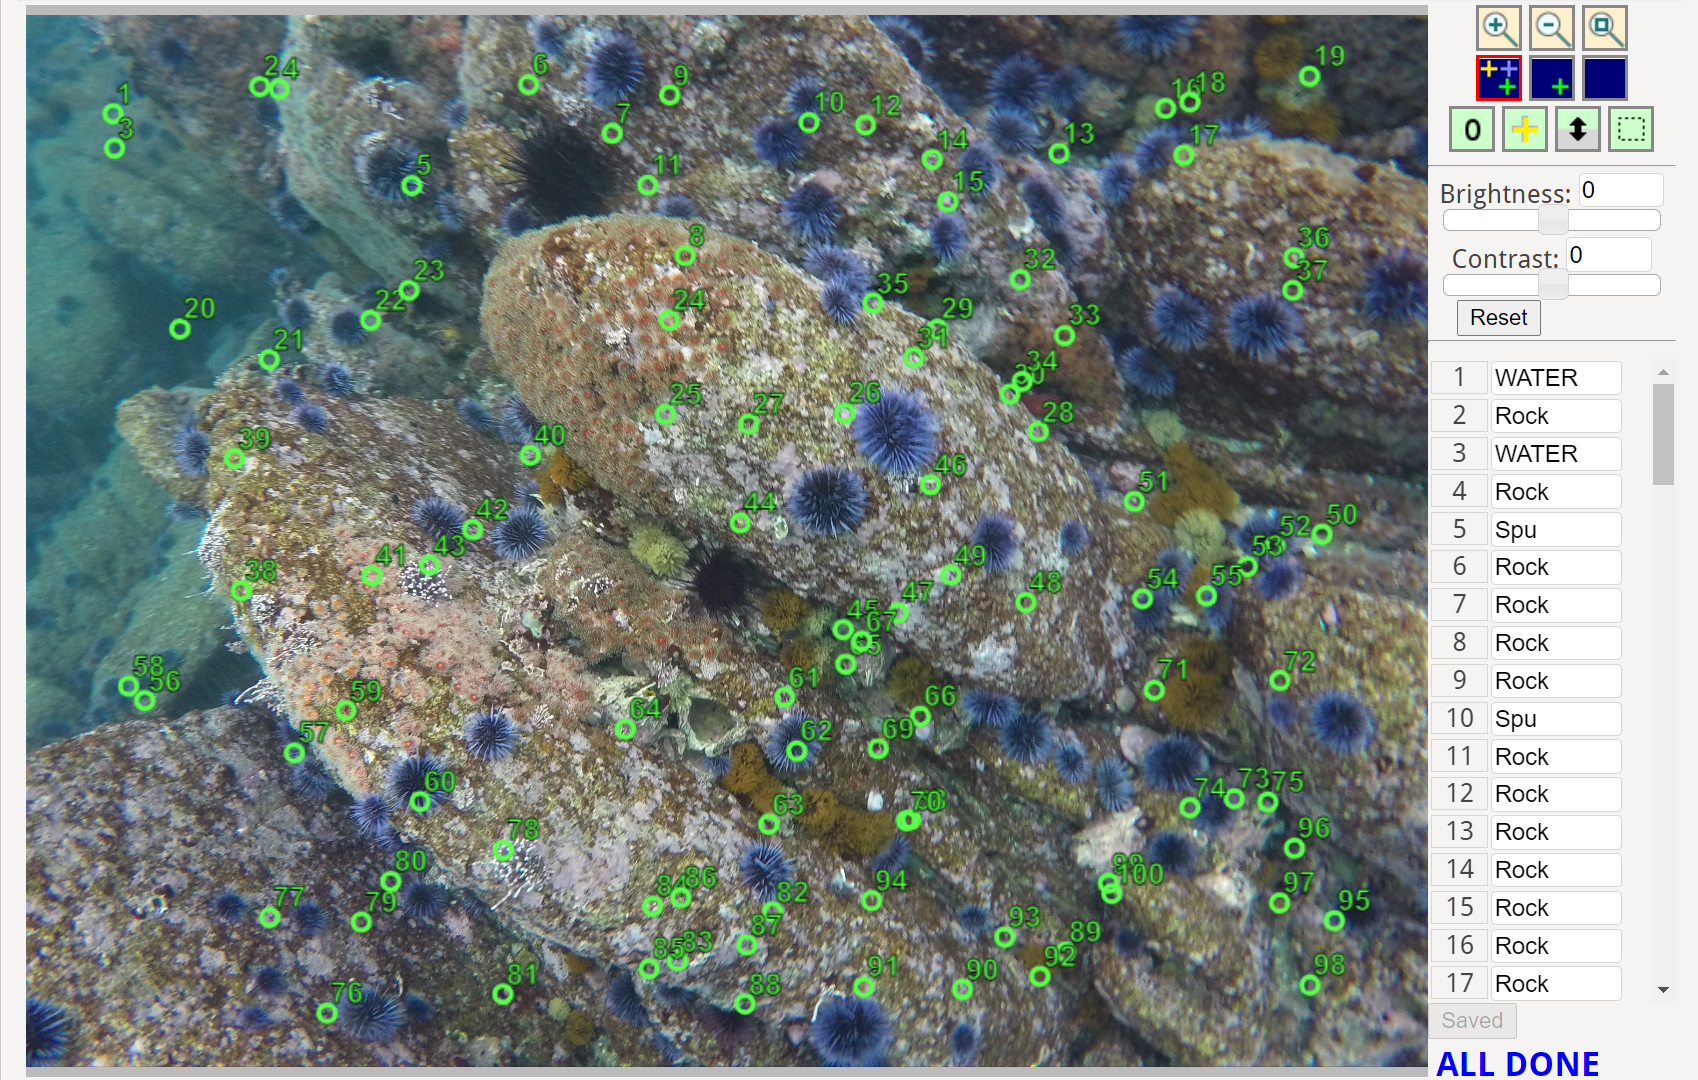
\includegraphics[
width=.5\textwidth, valign=t]{CoralNet1.png}}
\subfloat[]{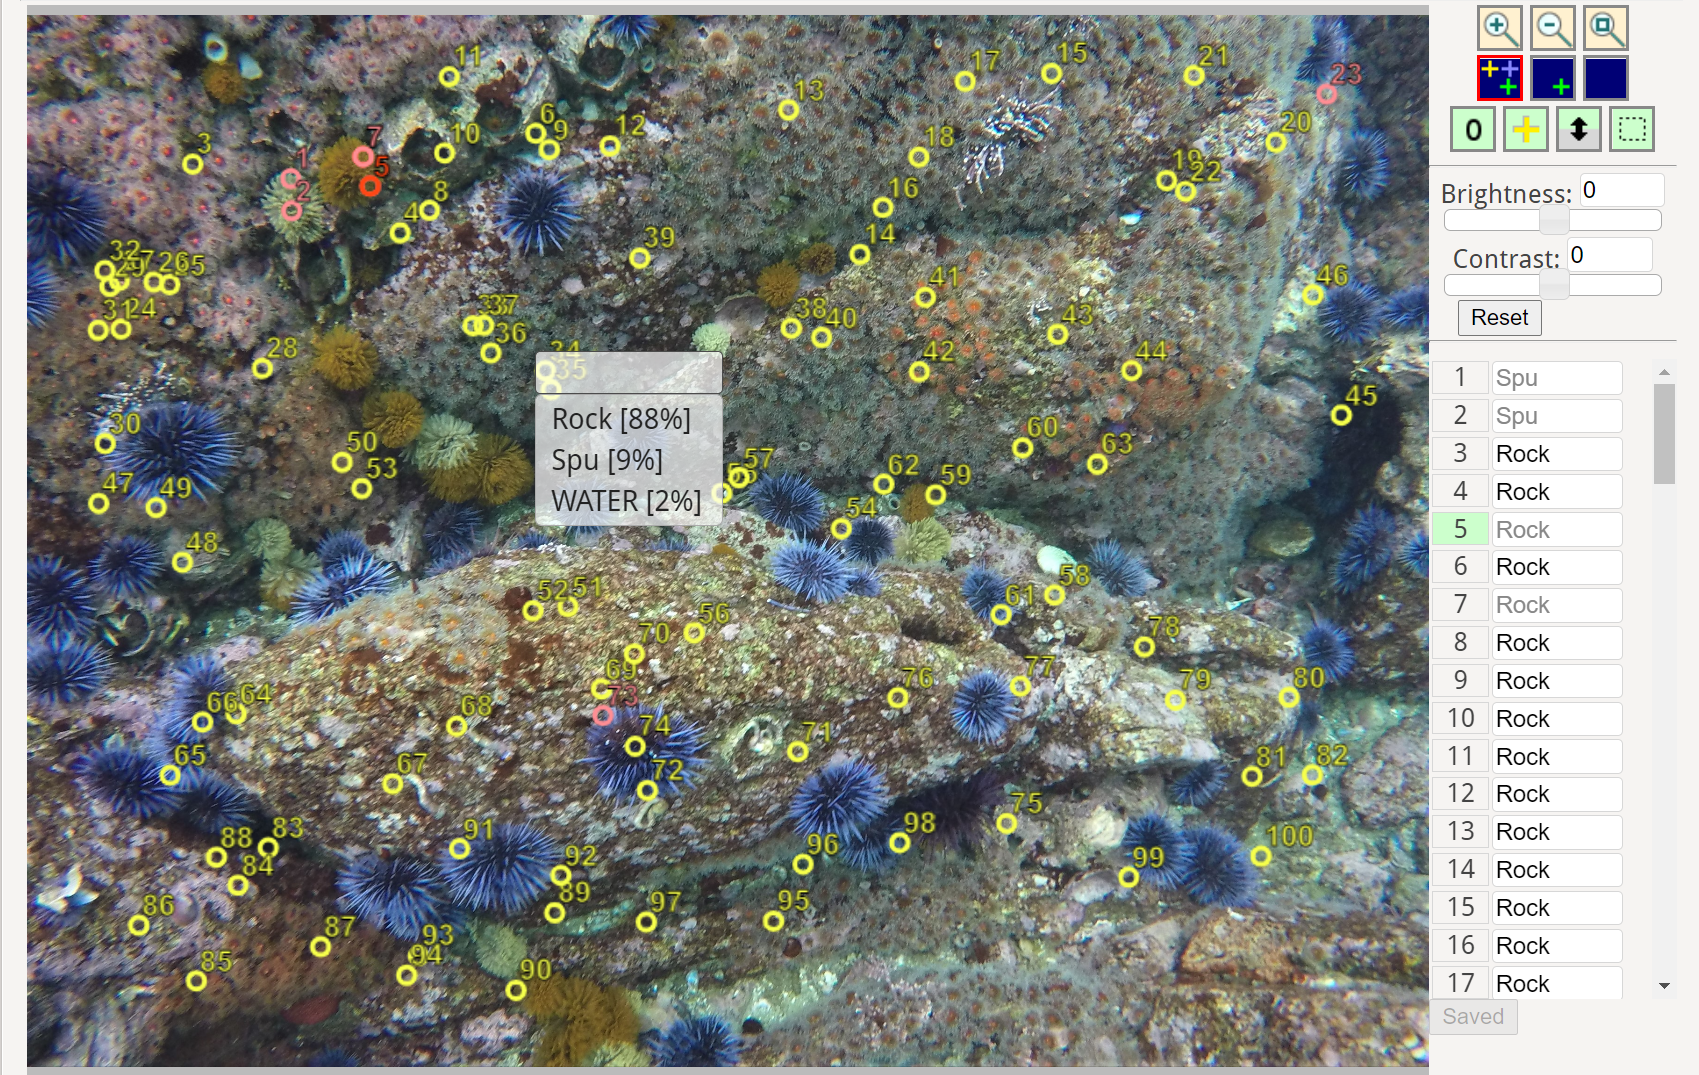
\includegraphics[
width=.5\textwidth, valign=t]{CoralNet2.png}}
\caption{
(\textit{a}) Screenshot of an image that has been manually annotated, 
i.e., an observer has selected a cover category for each of the 100 
randomly placed green circles. 
(\textit{b}) Screenshot of an image that has been annotated by the 
trained algorithm, i.e., the computer makes its best guess for what the 
category underlying each circle is. 
Yellow circles have been confirmed by an observer, and the red point 
that is selected (upper left) displays the percent confidence of the 
algorithm's predictions.
Selecting a point also provides the opportunity to correct the 
prediction, which in turn increases the accuracy of future 
predictions.  
}
\label{CoralNet}
\end{figure}

\subsection{Object detection via VIAME}
Video and Image Analytics for Multiple Environments (VIAME) is an 
open-source AI toolkit developed by Kitware with funding from NOAA. 
Here are links to an 
\href{https://www.viametoolkit.org/wp-content/uploads/2020/09/VIAME-AI-Workshop-Aug2020.pdf}{overview
 document}, a 
\href{https://viame.readthedocs.io/en/latest/index.html}{website} 
linking to most all VIAME information, and the 
\href{https://viame.kitware.com/#/}{VIAME online interface}. 
VIAME is open-source on 
\href{https://github.com/viame/VIAME}{GitHub}. 
Thus far I have opted to use the desktop version of VIAME, opposed 
to the online interface. 
This is because the desktop version provides access to all project 
files, whereas the online version automates the process and renders 
project files inaccessible. 
While there are extra considerations (and responsibilities) when 
managing project files, I opted for this so that we have the option to 
make our algorithms open-source, e.g., on GitHub.  
This will ensure anyone can download (but not change) our files, i.e., 
anyone can make use of the trained algorithm.

Shoutout to Olivia Rhoades, a postdoc with the Hakai Initiative in 
British Columbia, and Kathleen MacGregor, Aquatic Science Technician 
with Fisheries and Oceans Canada, Quebec, for providing me video and 
time-lapse photography (e.g., Fig.~\ref{VIAME}\textit{a,b}) of urchins 
in an urchin barren. 
These urchin-barren video and time-lapse photos were suited for 
investigation with VIAME, and they allowed me to develop the 
following proof-of-concept pipeline using VIAME. 

I first manually annotated half of a sequence of time-lapse images 
(Fig.~\ref{VIAME}\textit{c}).
This ``training" phase provided the information used to compile an 
algorithm---given our annotations---that can then be applied to other, 
unseen data. 
Annotations in VIAME involve creating a box around each observation of 
an object (e.g., an urchin, a crab, etc.), and correcting the position 
of the box as the object moves through the time-lapse or video.
VIAME has an option to automatically track the object in question, so 
following an individual through an image sequence is quick and easy. 
See 
\href{https://drive.google.com/file/d/12ubZDY16TSiEoi-b2XBXuypyJKBuxcDt/view?usp=sharing}{Vid.~4}
 for a screen-recording that scrolls through a sequence of 
 manually-annotated images.
(And note VIAME works perfectly well for ``single-detections", i.e., a 
single observation of an object).   
To test VIAME's ability to differentiate conspicuously visible versus 
cryptic individuals, I broke the category ``urchin" into $urchin$ (the 
urchin is clearly visible) and $covered\_urchin$ (urchins with 
decorations, e.g., rocks, algae, etc., on their test/spines). 
Many $covered\_urchins$ had no actual spines or parts of their 
test visible, and as they often looked identical to small rock piles, 
they were ideally suited to test VIAME's ability to differentiate 
cryptic species.
I furthermore annotated the movements of two very small sea stars 
to test how well VIAME handled tiny species comprised of relatively 
few pixels 
(\href{https://drive.google.com/file/d/1Hl3GFk9CDltWZcu24yrjcqk80Kb1c5TG/view?usp=sharing}{Vid.~5}).

With annotations in place, I compiled the annotations into a trained 
algorithm (a pipeline).
I opted to train a SVM (support-vector machine) model. 
One of the advantages of supervised SVM models is their ability to 
compile rather quickly---it took 17:03$min$ for my annotations to be 
compiled into a usable algorithm.
In contrast, Deep Learning or Convolutional Neural Network (CNN) models 
could take several days if not a week to initially train from a set of 
annotations.
(VIAME can train CNN models, and we will explore these 
once we have a more robust set of training annotations).  
Applying our trained SVM algorithm to unseen data (the other half of 
the time-lapse sequence) took 11:25$min$.
Given that we only had 100 individuals annotated across approximately 
80 frames (photos), the algorithm performed surprisingly well when 
applied to unseen imagery (Fig.~\ref{VIAME}\textit{d}).
See 
\href{https://drive.google.com/file/d/19CX6PiMXqZJvxj-YfzpFJOQLl5WSqlta/view?usp=sharing}{Vid.~6}
for a screen-recording of the classified output, i.e., of output from 
applying the algorithm to unseen data;
I scroll through frames from the time-lapse, and also scroll through \% 
confidence, a setting that filters predictions based on how confident 
the algorithm is regarding each detection. 

\begin{figure}[h!]
\centering
\subfloat[]{\includegraphics[
width=\ww, height=\hh, valign=t]{rawTimeLapse.png}}
\subfloat[]{\includegraphics[
width=\ww, height=\hh, valign=t]{whiteBalancedTimeLapse.png}}
\\
\subfloat[]{\includegraphics[
width=\ww, height=\hh, valign=t]{manualAnnotations.png}}
\subfloat[]{\includegraphics[
width=\ww, height=\hh, valign=t]{objectDetection.png}}
\caption{
(\textit{a}) Screenshot of raw image as I received it from Kathleen 
MacGregor, who staged a GoPro that took a photo every 1$min$.
(\textit{b}) Screenshot of same image after adjusting the white 
balance. 
(\textit{c}) Screenshot of VIAME while creating manual annotations, 
i.e., ``informing" the computer what an urchin is, what a crab is, etc.
(\textit{d}) Screenshot of the trained algorithm applied to unseen 
data, i.e., the algorithm's attempt at identifying species given the 
manual annotations we provided. 
}
\label{VIAME}
\end{figure}

Finally, data from annotating and then applying an algorithm are easy 
to work with via exported CSV files.  
As as example, Fig.~\ref{movement} presents the tracking data generated 
from annotating the urchin-barren imagery. 
Each ``line" represents a single individual (urchin, crab, etc.) 
tracked across the entirety of the training sequence
(Fig.~\ref{movement}\textit{a}). 
Fig.~\ref{movement}\textit{b} visualizes the kernal densities of 
individual step-lengths for \textit{urchins} and 
\textit{covered$\_$urchins} (with step-length distance in $mm$ that 
have been log base-10 transformed).
We see \textit{covered$\_$urchin} exhibit a higher frequency of short 
steps, whereas \textit{urchins} predominantly exhibit the longer 
step-lengths. 
If we wanted to test for differences between these kernal densities 
(distributions), we could use a two-way Kolmogorov-Smirnov Test. 
Finally, note that we could also incorporate urchin size information 
(based on the size of VIAME's bounding box around each observation) to 
model the urchin-size vs step-length relationship. 

\begin{figure}[!]
\centering
\subfloat[]{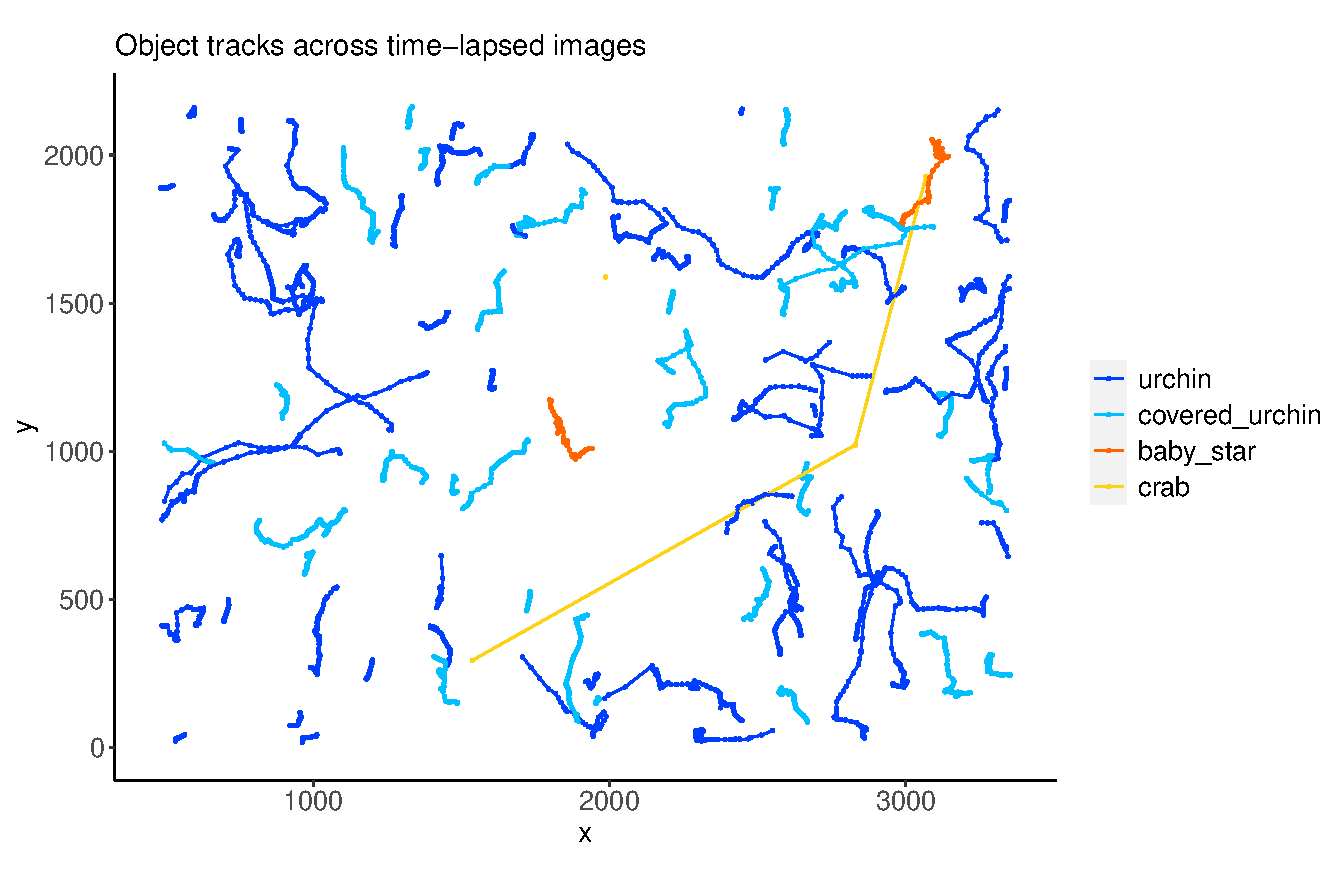
\includegraphics[
width=.5\textwidth, valign=t]{tracks.pdf}}
\subfloat[]{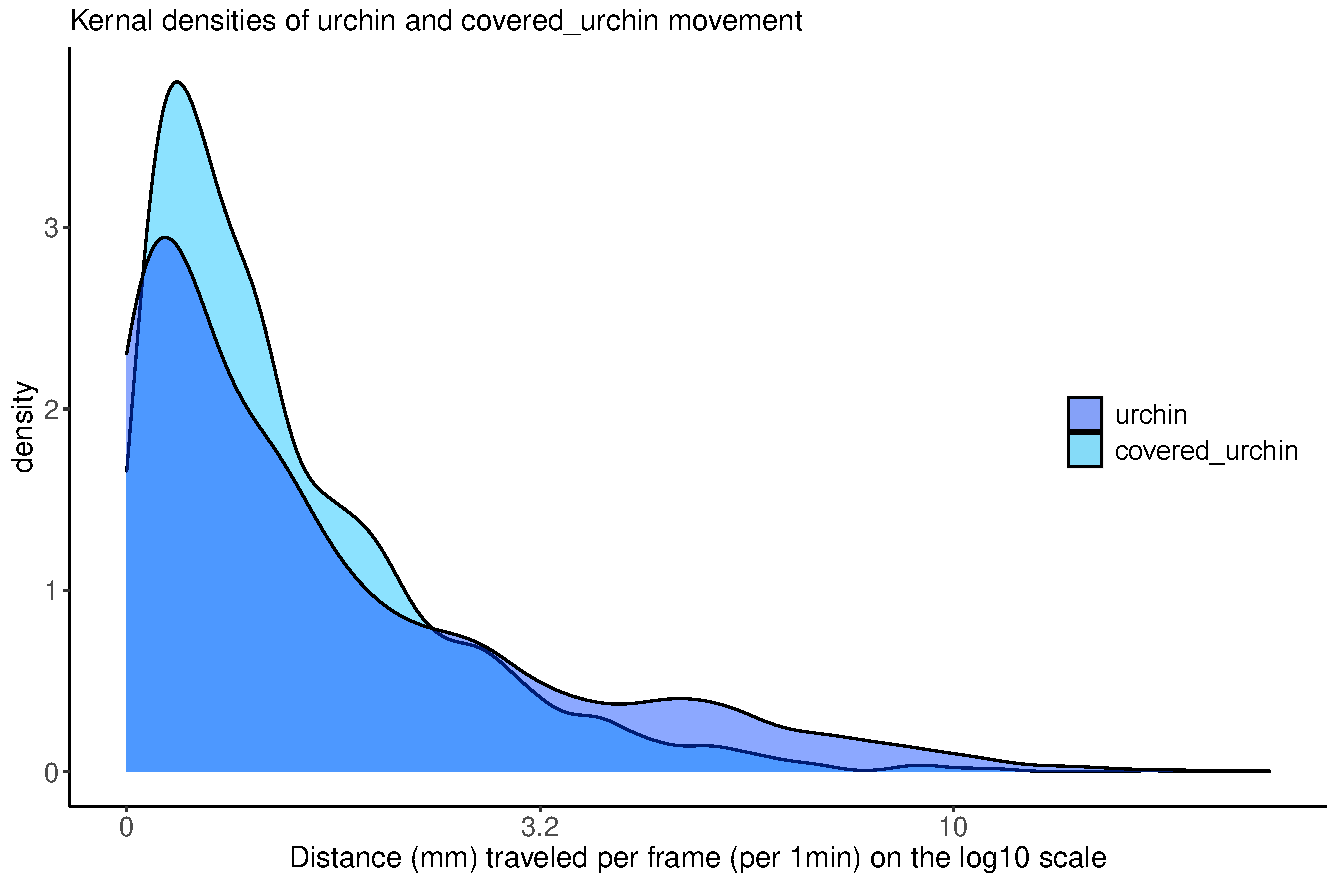
\includegraphics[
width=.5\textwidth, valign=t]{density.pdf}}
\caption{
(\textit{a}) Movement tracks of individuals from the four categories of 
species: \textit{urchin}, \textit{covered$\_$urchin}, 
\textit{crab}, and \textit{baby$\_$star}. 
(Note a large \textit{crab} was observed in three sequential images 
before moving out of frame, hence the two long and 
straight lines connecting each of the three observations). 
(\textit{b}) Movement patterns summarized with kernal densities for 
\textit{urchin} and \textit{covered$\_$urchin}, with the former 
exhibiting high frequencies of longer movements (with step-length in 
$mm$ and log base-10 transformed).
}
\label{movement}
\end{figure}

\subsection{Next steps re: AI analyses}
\begin{itemize}
\pt
\item In order to establish version-control and enable accessible 
research, I have created a GitHub repository (a repo) with all 
necessary files to run the VIAME algorithm trained here. 
This GitHub repo--- 
\href{https://github.com/zhrandell/AI\_proofOfConcept}{https://github.com/zhrandell/AI$\_$proofOfConcept}---is
 currently set to ``public", so anyone can access and 
download the files. 
However, these files are only usable if one has downloaded VIAME.
Furthermore, this repo will be more useful when I can upload imagery so 
that one can reproduce the process of training an algorithm (I have not 
yet received permission to publicly release the images I used). 
Additional future action items include creating tutorial content: with 
a Zoom recording, I will talk through and screenshare the steps of 
``pulling" from and ``pushing" to a GitHub repository, downloading 
VIAME, training an algorithm, applying a trained pipeline, etc.
\pt
\item Next steps with CoralNet include using ROV-obtained images to 
create and classify real categories of interest, e.g., red algae, brown 
algae, colonial/aggregate invertebrates, and substrate type (as 
described in the CoralNet subsection \ref{CoralNet}).
\pt
\item Next steps with VIAME (similar to CoralNet) involve training an 
algorithm on ROV-derived imagery. 
Additionally, there are other photogrammetry tools in VIAME (such as 
the ability to generate photo mosaics) that will be worth exploring.
\pt
\item Finally, once a robust training set of images have been annotated 
in VIAME, we will compile deep learning or CNN models. 
\end{itemize}
%% END AI analyses ~~~~~~~~~~~~~~~~~~~~~~~~~~~~~~~~~~~~~~~~~~~~~~~~~~ %%





%% END document ~~~~~~~~~~~~~~~~~~~~~~~~~~~~~~~~~~~~~~~~~~~~~~~~~~~~~ %%
\end{document}
%% END document ~~~~~~~~~~~~~~~~~~~~~~~~~~~~~~~~~~~~~~~~~~~~~~~~~~~~~ %%
